 %
% Niniejszy plik stanowi przykład formatowania pracy magisterskiej na
% Wydziale MIM UW.  Szkielet użytych poleceń można wykorzystywać do
% woli, np. formatujac wlasna prace.
%
% Zawartosc merytoryczna stanowi oryginalnosiagniecie
% naukowosciowe Marcina Wolinskiego.  Wszelkie prawa zastrzeżone.
%
% Copyright (c) 2001 by Marcin Woliński <M.Wolinski@gust.org.pl>
% Poprawki spowodowane zmianami przepisów - Marcin Szczuka, 1.10.2004
% Poprawki spowodowane zmianami przepisow i ujednolicenie 
% - Seweryn Karłowicz, 05.05.2006
% Dodanie wielu autorów i tłumaczenia na angielski - Kuba Pochrybniak, 29.11.2016

% dodaj opcję [licencjacka] dla pracy licencjackiej
% dodaj opcję [en] dla wersji angielskiej (mogą być obie: [licencjacka,en])
\documentclass[en]{pracamgr}

% Dane magistranta:
\autor{Adam Starak}{361021}

\title{Application of parameterized techniques to finding spanning star forests in graphs}
\titlepl{Zastosowanie technik algorytmów parametryzowanych dla problemu znajdowania  rozpinających lasów gwiazd w grafach}

%\tytulang{An implementation of a difference blabalizer based on the theory of $\sigma$ -- $\rho$ phetors}

%kierunek: 
% - matematyka, informacyka, ...
% - Mathematics, Computer Science, ...
\kierunek{Computer Science}

% informatyka - nie okreslamy zakresu (opcja zakomentowana)
% matematyka - zakres moze pozostac nieokreslony,
% a jesli ma byc okreslony dla pracy mgr,
% to przyjmuje jedna z wartosci:
% {metod matematycznych w finansach}
% {metod matematycznych w ubezpieczeniach}
% {matematyki stosowanej}
% {nauczania matematyki}
% Dla pracy licencjackiej mamy natomiast
% mozliwosc wpisania takiej wartosci zakresu:
% {Jednoczesnych Studiow Ekonomiczno--Matematycznych}

% \zakres{Tu wpisac, jesli trzeba, jedna z opcji podanych wyzej}

% Praca wykonana pod kierunkiem:
% (podać tytuł/stopień imię i nazwisko opiekuna
% Instytut
% ew. Wydział ew. Uczelnia (jeżeli nie MIM UW))
\opiekun{dr Michał Pilipczuk\\
  Institute of Informatics\\
  }

% miesiąc i~rok:
\date{\monthyeardate\today}

%Podać dziedzinę wg klasyfikacji Socrates-Erasmus:
\dziedzina{ 
%11.0 Matematyka, Informatyka:\\ 
%11.1 Matematyka\\ 
%11.2 Statystyka\\ 
11.3  Informatics, Computer Science \\
%11.4 Sztuczna inteligencja\\ 
%11.5 Nauki aktuarialne\\
%11.9 Inne nauki matematyczne i informatyczne
}

%Klasyfikacja tematyczna wedlug AMS (matematyka) lub ACM (informatyka)

\klasyfikacja{ Theory of computation $\rightarrow$ Parameterized complexity and exact algorithms}

% Słowa kluczowe:
\keywords{parameterized algorithm, kernelization, Strong Expotential-Time Hypothesis, tree decomposition, cross-composition}

% Tu jest dobre miejsce na Twoje własne makra i~środowiska:

\usepackage{chngcntr}
\usepackage{amsthm}
\usepackage{amsmath}
\usepackage[]{algorithm2e}
\usepackage{enumitem}
\usepackage{datetime}
\usepackage{amssymb}
\usepackage{thmtools}
\usepackage{thm-restate}
\usepackage{hyperref}
\usepackage{cleveref}
\usepackage{tikz}

\usetikzlibrary{positioning,shapes,calc,fit}

\newdateformat{monthyeardate}{%
	\monthname[\THEMONTH], \THEYEAR}

\newtheorem{theorem}{Theorem}
\newtheorem{lemma}{Lemma}
\newtheorem{claim}{Claim}
\newtheorem{corollary}{Corollary}
\newtheorem{proposition}{Proposition}
\newtheorem{conjecture}{Conjecture}

\theoremstyle{definition}
\newtheorem{definition}{Definition}

\newcommand{\wcs}{Weighted Circuit Satisfiability}

\newenvironment{sproof}{%
	\renewcommand{\proofname}{Proof (sketch).}\proof}{\endproof}

\newcommand{\ssf}{spanning star forest}
\newcommand{\ssfp}{{\sc Spanning Star Forest}}
\newcommand{\dssfp}{{\sc Decision Spanning Star Forest}}
\newcommand{\mssfp}{{\sc Minimal Spanning Star Forest}}
\newcommand{\ssfep}{{\sc Spanning Star Forest Extension}}
\newcommand{\domset}{dominating set}
\newcommand{\domsetp}{{\sc Dominating Set}}
\newcommand{\indset}{{\sc Independent Set}}
\newcommand{\cnfsat}{{\sc CNF-SAT}}

\newcommand{\degree}[2]{\textrm{deg}_{#1}(#2)}
\newcommand{\dpt}[1]{\textrm{dp}[#1]}
\newcommand{\true}{\textrm{True}}
\newcommand{\false}{\textrm{False}}
\newcommand{\tw}{\textrm{tw}}
\newcommand{\w}[1]{\textrm{W}[#1]}
\DeclareMathOperator{\Ima}{Im}

\newcommand{\kssf}{\emph{Spanning Star Forest Problem} parameterized by the number of stars}
\newcommand{\ssfe}{\emph{Spanning Star Forest Extension Problem}}
\newcommand{\tsat}{\emph{3-SAT}}

\counterwithin{theorem}{chapter}
\counterwithin{definition}{chapter}
\counterwithin{lemma}{chapter}
\counterwithin{corollary}{chapter}
\counterwithin{claim}{chapter}
\counterwithin{proposition}{chapter}
\counterwithin{conjecture}{chapter}

% koniec definicji

\begin{document}
\maketitle

%tu idzie streszczenie na strone poczatkowa
\begin{abstract}
	We present applications of parameterized techniques to the problem of finding spanning star forests in graphs. We examine three different variants of the problem and multiple parametrizations. We present positive results such as parameterized algorithms, kernelization procedures, algorithms over a tree decomposition of an input graph as well as negative ones, like hardness results based on the Strong Exponential-Time Hypothesis.
\end{abstract}

\tableofcontents
%\listoffigures
%\listoftables

\chapter{Introduction}

A spanning star forest of a graph is a subgraph that contains all the vertices and any connected component is a tree of depth $2$. Note that we do not allow isolated vertices in a spanning star forest. In the \ssfp{} problem, given a graph, we ask whether there exists a spanning star forest. 

The goal of this paper is to apply numerous parameterized techniques to three different variants of the problem. We start with the most basic variant, denoted \ssfp{} where we only ask whether a graph has a spanning star forest. We show a simple condition, verifiable in linear time, that is necessary and sufficient for the existence of a spanning star forest in a graph. Later, we present a linear time algorithm that constructs a spanning star forest. The following theorem summarizes these results:

\begin{restatable}{theorem}{thmssfp}\label{thm-ssfp}
	\ssfp{} can be solved in linear time. Moreover, given a graph $G$, one can find a solution in linear time if it exists.
\end{restatable}

Afterwards, we introduce the second variant. In \mssfp{}, we look for a spanning star forest with the minimum possible number of stars. We show that \mssfp{} and \domsetp{} are essentially equivalent. That is, they are interreducible with respect to parameterized and polynomial-time reductions. Thus, we obtain the following outcomes:

\begin{restatable}{theorem}{thmmssfpwc}\label{thm-mssfp-w2c}
	\mssfp{} parameterized by the number of stars is \textup{W[2]}-complete.
\end{restatable}

\begin{restatable}{theorem}{thmmssfpnpc}\label{thm-mssfp-npc}
	\mssfp{} is \textup{NP-complete}.
\end{restatable}

\noindent
Based on reductions, we show a brute force algorithm. We point out that its running time is tight, using a lower bound proved for \domsetp{} by Pătraşcu and Williams \cite{DomSet}. 

\begin{restatable}{theorem}{thmmssfptime}\label{thm-mssfp-time}
	\mssfp{} can be solved in $\mathcal{O}^*(N^{k + o_k(1)})$, where $N$ is the number of vertices.
\end{restatable}

\begin{restatable}{theorem}{thmmssfplowerbound}\label{thm-mssfp-lowerbound}
	Unless \cnfsat{} can be solved in time $\mathcal{O}^*((2-\epsilon')^n)$
	\footnote{The notation $\mathcal{O}^*$ is commonly used when stating the running times of parameterized algorithms. The notation hides polynomial factors.}
	 for some $\epsilon' > 0$, there does not exist constants $\epsilon > 0,k\geq 7$ and an algorithm solving \mssfp{} on instance with parameter equal to $k$ in time $\mathcal{O}(N^{k-\epsilon})$, where $N$ is the number of vertices of the graph.
\end{restatable}

Finally, we introduce the last variant. In \ssfep{} we are given a graph and a subset of forced edges. We ask whether there exists a spanning star forest in the graph that extends the subset of forced edges. By free vertices we mean vertices that are not adjacent to any forced edge. We prove that this problem is essentially equivalent to \cnfsat{}, where the number of forced edges corresponds to the number of variables, while the number of free vertices corresponds to the number of clauses. Thus, we obtain:

\begin{restatable}{theorem}{thmssfepnpc}\label{thm-ssfep-npc}
	\ssfep{} is \textup{NP}-complete.
\end{restatable}

\noindent
For the parametrization by the number of forced edges, our reductions yield the following:

\begin{restatable}{theorem}{thmssfepfetime}\label{thm-ssfep-fe-time}
	\ssfep{} parameterized by the number of forced edges can be solved in time $\mathcal{O}^*(2^{|F|})$ where $|F|$ is the number of forced edges.
\end{restatable}

\begin{restatable}{theorem}{thmssfepseth}\label{thm-ssfep-seth}
	For every $\epsilon > 0$, there exists an algorithm solving \cnfsat{} in time $\mathcal{O}^*((2-\epsilon)^n)$ where $n$ is the number of variables if and only if there exists an algorithm solving \ssfep{} parameterized by the number of forced edges in time $\mathcal{O}^*((2-\epsilon)^n)$ where $n$ is the number of forced edges.
\end{restatable}

\noindent
Also, we argue that there does not exist a polynomial kernel for \ssfep{} when parameterized by the number of forced edges unless NP $\subseteq$ coNP/poly. We show two different approaches. The first one uses \cnfsat{} and its hardness of kernelization. In the second approach, we apply the composition framework proposed by Bodlaender~et~al.~\cite{Bodlaender}. Namely, we prove that there exists a cross-composition of \ssfep{} into itself. All in all, we obtain the following result:

\begin{restatable}{theorem}{thmssfepnokernel}\label{thm-ssfep-nokernel}
	\ssfep{} parameterized by the number of forced edges does not admit a polynomial kernel unless NP $\subseteq$ coNP/poly.
\end{restatable}

Recall that our reductions provides a link between free vertices and clauses. Therefore, when we parameterize the problem by the number of free vertices, we can immediately transfer the algorithm for \cnfsat{} parameterized by the number of clauses proposed by Bliznets and Golovnev \cite{MAXSAT} and obtain the following:

\begin{restatable}{theorem}{thmssfepfreealg}\label{thm-ssfep-free-alg}
	\ssfep{} can be solved in time $\mathcal{O}^*(1.358^k)$ where $k$ is the number of free vertices.
\end{restatable}

\noindent
Furthermore, unlike in the case of the previous parametrization, we provide an algorithm that outputs a linear kernel.

\begin{restatable}{theorem}{thmssfepkernel}\label{thm-ssfep-kernel}
	\ssfep{} parameterized by the number of free vertices admits a kernel with at most $k$ free vertices and at most $k$ forced edges.
\end{restatable}

Finally, we study the parameterization of the extension variant by the width of the given tree decomposition. We propose a dynamic programming algorithm over a decomposition of a graph which uses fast cover product computation proposed by Björklund et al. \cite{CoverProduct}. In addition, we show that improving the running time would give a faster algorithm for the \cnfsat{} problem.

\begin{restatable}{theorem}{thmssfeptwtime}\label{thm-ssfep-tw-time}
	\ssfep{} can be solved in time $2^w\cdot poly(w)\cdot n$, where $w$ is the width of a given tree decomposition.
\end{restatable}

\begin{restatable}{theorem}{thmssfeptwseth}\label{thm-ssfep-tw-seth}
	Unless \cnfsat{} can be solved in time $\mathcal{O}^*((2-\epsilon)^n)$ for some $\epsilon > 0$, there is no algorithm for \ssfep{} that would achieve running time $\mathcal{O}^*((2-\epsilon)^{w})$ for any $\epsilon > 0$, where $w$ is the width of a given tree decomposition.
\end{restatable}

\paragraph{Outline.} In Section 2 we present notation and recall basic definitions related to parameterized complexity. Section 3 contains results for \ssfp{}. In Section 4 we prove all the theorems about \mssfp{}. Section 5 gives the algorithms and lower bounds for \ssfep{} parameterized in three different ways.

\chapter{Preliminaries}\label{sec2}

\section{Structures}

In a simple graph $G$ we denote by $V(G)$ and $E(G)$ the sets of vertices and of edges, respectively. 
Let $\degree{G}{v}$ denote degree of the vertex $v$ in the graph $G$ which is the number of adjacent vertices. 
An induced graph $G'$ of $G$ is a subgraph formed from a subset of vertices and all the edges between them that are present in $G$. 
For a set $X \subseteq V(G)$, by $G[X]$ we define the graph induced by vertices from $X$. 
Let $G \setminus v$ be the abbreviation for $G[V(G) \setminus \{v\}]$.
$G'$ is a \emph{subgraph} of $G$, denoted by $G' \subseteq G$, if $V(G') \subseteq V(G)$ and $E(G') \subseteq E(G)$.
A \emph{tree} $T$ is a connected graph which has exactly $|V(T)|-1$ edges. 
A \emph{spanning tree} $T$ of a graph $G$ is a connected subgraph which includes all of the vertices of $G$, with the minimum possible number of edges.
A \emph{star} $S$ is a tree with at least $2$ vertices in which at most one vertex has a degree greater than $1$. 
A star of size at least $3$ consists of a \emph{center}, that is a vertex of the greatest degree, and \emph{rays} --- vertices of degree $1$. 
Vertices of a star of size 2 are called \emph{candidates}.
For a given graph $G$, we say that $S$ is a \emph{\ssf{}} if $V(S)=V(G)$ and every connected component of $S$ is a star.

\section{Parameterized complexity}

\emph{Parameterized complexity} is a young branch of computational complexity theory. We refer the reader to textbooks of Downey and Fellows \cite{ParComp}, Flum and Grohe \cite{ParCompThm} and Cygan et al. \cite{ParAlg} for an overview of the field.

We now introduce basic terminology. We begin with formally defining a parameterized problem. For the sake of clarity, all the definitions are taken from \cite{ParAlg}.

\begin{definition}\label{Parameterized problem}
	A \textit{parameterized problem} is a language $L \subseteq \Sigma^* \times \mathbf{N}$, where $\Sigma$ is a fixed, finite alphabet. For an instance $(x,k) \in L$, $k$ is called the \textit{parameter}.
\end{definition}

\noindent
Consider the example problems:

\begin{definition}
	\indset{}: Given a graph $G$ and a positive integer $k$, decide whether there exists a set $I$ such that $|I|=k$ and $G[I]$ has no edges.
\end{definition}

\begin{definition}
	\domsetp{}: Given a graph $G$ and a positive integer $k$, decide whether there exists a set $D$ such that $|D| \leq k$ and every vertex is either in $D$ or is adjacent to one of the vertices from $D$.
\end{definition}

There are multiple different parameters for a single problem. For example, \domsetp{} can be parameterized by the sought size of dominating set or by the treewidth of the input graph. 

Now, we want to introduce different complexity classes. The first one is called FPT (fixed parameter tractable). We say that a parameterized problem is in FPT if and only if it has an FPT algorithm defined below:

\begin{definition}\label{FPT algorithm}
	For a parameterized problem $Q$, an \textit{FPT algorithm} is an algorithm $\mathcal{A}$ which, for every input $(x,k)$, decides whether $(x,k) \in Q$ in time $f(k)\cdot n^c$ where c is a constant, independent of $n,k$, and $f$ is a computable function.
\end{definition}

\noindent
Another important class of parameterized problems is XP. Similarly, a problem is in XP if and only if it has an XP algorithm defined below:

\begin{definition}
	For a parameterized problem $Q$, an \textit{XP algorithm} is an algorithm $\mathcal{A}$ which, for any input $(x,k)$, decides whether $(x,k) \in Q$ in time $n^{f(k)}$ where $f$ is a computable function.
\end{definition}

Similarly to polynomial-time reductions, we now introduce a \textit{parameterized reduction}, that is, a notion of transforming instances of a certain parameterized problem to instances of another one.

\begin{definition}
	Let $P,Q \subseteq \Sigma^* \times \mathbb{N}$ be two parameterized languages. A  \textit{parameterized reduction} from $P$ to $Q$ is an algorithm $\mathcal{A}$ that given $(x,k) \in P$ outputs $(x',k') \in Q$ such that the following three conditions hold:
	\begin{enumerate}
		\item $(x,k)$ is a YES-instance of $P$ if and only if $(x',k')$ is a YES-instance of $Q$.
		\item $k' \leq g(k)$ for some computable function $g$.
		\item The running time of $\mathcal{A}$ is $f(k) \cdot |x^c|$ for some computable function $f$ and constant $c$.
	\end{enumerate}
\end{definition}

Finally, we introduce the last family of complexity classes. \emph{W-hierarchy} is an ascending chain of classes : $\w{1} \subseteq \w{2} \subseteq \w{3} \subseteq...$ . For the purpose of this paper, we define \w{1} as the closure of the \indset{} problem and \w{2} as the closure of the \domsetp{} problem under parameterized reductions. In other words, \indset{} parameterized by the size of independent set is  \w{1}-complete and \domsetp{} parameterized by the size of dominating set is \w{2}-complete with respect to parameterized reductions. It is known that $\textrm{FPT} \subseteq \w{1}$ and it is conjectured that this containment is strict.

Last but not least, we introduce a \emph{kernelization algorithm} --- a way of reducing the size of input instances in polynomial time:

\begin{definition}\label{Kernel}
	A \textit{kernel} for a parameterized problem $Q$ is an algorithm $\mathcal{A}$ that, given an instance $(x,k)$ of $Q$, works in polynomial time and returns an equivalent instance $(x',k')$ of $Q$
	such that $|x'| + k' \leq g(k)$ for a computable function $g$, called the \textit{size} of the kernel.
\end{definition}

\section{Tree decomposition}

Formally, a tree decomposition of a graph $G$ is a pair $\mathcal{T} = (T, \{X_t\}_{t\in V(T)})$ where $\mathcal{T}$ is a tree whose every node $t$ is assigned a vertex subset $X_t \subseteq V(G)$, called a \emph{bag}, such that the following three conditions hold:
\begin{itemize}
	\item[(T1)] $\bigcup_{t\in V(T)}X_t = V(G)$.
	\item[(T2)] For every $vu \in E(G)$ there exists a node $t$ of $\mathcal{T}$ such that $v,u \in X_t$.
	\item[(T3)] For every $v \in V(G)$ the set $T_v = \{t \in V(T): v \in X_t\}$ induces a connected subtree of $\mathcal{T}$.
\end{itemize}

The \emph{width} of a tree decomposition $\mathcal{T} = (T,\{X_t\}_{t\in V(T)})$, denoted $\textrm{tw}(\mathcal{T})$, is equal to $\max_{t \in V(T)} |X_t| - 1$. The treewidth of a graph $G$, denoted $\textrm{tw}(G)$, is the minimum width over all tree decompositions of $G$.
\\\\
A \emph{nice tree decomposition} of a graph $G$ is a tree decomposition $(T, \{X_t\}_{t \in V(T)})$, where $T$ is rooted, such that:
\begin{itemize}
	\item $X_i = \emptyset$ if $i$ is either the root or a leaf.
	\item Every non-leaf node is of one of the three following types:
	\begin{itemize}
		\item \textbf{Introduce vertex node}: a node $t$ with exactly one child $t'$ such that $X_t = X_{t'} \cup \{v\}$ for some vertex $v \notin X_{t'}$.
		\item \textbf{Introduce edge node}: a node $t$ labeled with edge $vu \in V(G)$ such that $u,v \in X_t$ with exactly one child $t'$ such that $X_t = X_{t'}$.
		\item \textbf{Forget node}: a node $t$ with exactly one child $t'$ such that $X_t = X_{t'} \setminus \{v\}$ for some vertex $v \in X_{t'}$
		\item \textbf{Join node}: a node $t$ with exactly two children $t_1$, $t_2$ such that $X_t = X_{t_1} = X_{t_2}$.
	\end{itemize}
\end{itemize}
Note that every tree decomposition can be turned into a nice one without increasing the width in time $\textrm{poly}(t) \cdot n$ \cite{ParAlg}.

\iffalse
We distinguish one special case. If a tree $\mathcal{T}$ forms a path, we call it a \emph{path decomposition}. Respectively, by $\textrm{pw}(\mathcal{T})$ we denote a width of a path decomposition and by $\textrm{pw}(G)$ we denote the minimum width over all path decompositions of $G$.
\fi
\section{Satisfiability problem}

In this section we present the \cnfsat{} problem. We also recall two hypotheses about its complexity. They are fundamental for proving lower bounds on running times of algorithms. 

A \textit{conjunctive normal form} (CNF) of a propositional formula $\phi$ on $n$ Boolean variables $x_1,x_2,...,x_n$ is a formula of form $\phi=C_1 \land C_2 \land ... \land C_m$, where $C_i$ is a \textit{clause}. Each clause $C_i$ consists of disjunction of \textit{literals}, that is, $C_i=l_1 \lor l_2 \lor ... \lor l_j$. A literal $l_j$ corresponds to either a variable $x_k$ or its negation $\neg x_k$. We also introduce the abbreviation $l_i \in C_j$ which means that a literal $l_i$ occurs in $C_j$.

Now, we are ready to formally formulate the \cnfsat{} problem:

\begin{definition}
	\cnfsat{}: given a propositional formula $\phi$ on $n$ Boolean variables $x_1,x_2,...,x_n$ that is in conjunctive normal form, decide whether there exists an evaluation of variables $\sigma$, such that $\sigma(\phi)=\true$.
\end{definition}

\noindent
Note that by $\sigma(\phi)=\true$ we mean a satisfying assignment of variables for $\phi$.

It is worth mentioning one more variant of a satisfiability problem. By restricting the number of literals in clauses to some constant $q$ we arrive at the $q$-{\sc SAT} problem. Observe that for $q \geq 3$, $q$-{\sc SAT} is NP-Complete by Cook-Levin Theorem. Let $\delta_q$ be an infinimum of the set of constants $c$ for which there exists an algorithm solving $q$-{\sc SAT} in time $\mathcal{O}^*(2^{cn})$. The \textit{Exponential-Time Hypothesis} and \textit{Strong Exponential-Time Hypothesis} are defined as follows:

\begin{conjecture}[\textbf{Exponential-Time Hypothesis, ETH}]

\begin{equation*}
	\delta_3 > 0
\end{equation*}
\end{conjecture}

\begin{conjecture}[\textbf{Strong Exponential-Time Hypothesis, SETH}]\label{SETH}
	
	\begin{equation*}
	\lim\limits_{q \rightarrow \infty}\delta_q = 1
	\end{equation*}
\end{conjecture}

Intuitively, ETH states that we need to browse through an exponential number of assignments for $3$-{\sc SAT}, while SETH implies that as the number of literals in clauses grows, brute force check is inevitable. However, in this paper we do not refer directly to the above conjectures, but to the following consequence of Conjecture \ref{SETH}

\begin{conjecture}
	\cnfsat{} cannot be solved in time $\mathcal{O}^*((2-\epsilon)^n)$ for any $\epsilon>0$.
\end{conjecture}

\chapter{Spanning Star Forest Problem}\label{sec3}

In this chapter we examine both decision and constructive variant of \ssfp{}. We propose an algorithm working in linear time that outputs a \ssf{} or concludes that the given instance is a NO-instance.

\section{Decision variant}

In the decision variant of \ssfp{}, all that we have to do is to answer whether there exists a spanning star forest of an input graph. As it turns out, every graph that does not contain any isolated vertex has a \ssf{}.

\begin{lemma}\label{SSF lemma}
 A graph $G$ has a \ssf{} if and only if it does not contain any isolated vertices.
\end{lemma}

\begin{proof}
	If $G$ has a \ssf{} $S$, then we have that for all $v \in V(G),\ 1 \leq deg_S(v) \leq deg_G(v)$. Thus, none of the vertices is isolated.
	
	For the opposite direction, we prove the lemma by induction on $|V(G)|$. Assume $|V(G)|=2$. The statement trivially holds because a graph consisting of one edge and two vertices is a \ssf{}. Let $|V(G)| >2$. For the induction step, we split the proof into two parts. 
	
	Firstly, suppose that for all vertices $v \in V(G)$, it holds that $\degree{G}{v}=1$.  Clearly, $G$ is a matching. Hence, it is a \ssf{} by itself. 
	
	Now, suppose that there exists a vertex $u$ such that $\degree{G}{u}>1$. Let $C \subseteq G$ be the connected component satisfying $u \in V(C)$. Based on the degree of $u$, we infer that $|V(C)|>2$. Let $T$ be an arbitrary spanning tree of $C$ and $v$ be one of its leaf. Observe that $T \setminus v$ is a spanning tree of $C \setminus v$. So, $C \setminus v$ does not have any isolated vertices and neither has the graph $G \setminus v$. Now, from the induction, let $S$ be a \ssf{} of the graph $G \setminus v$, $u$ be a vertex such that $uv \in E(G)$ and let $w \in N_S(u)$. Consider the two following cases:
	\begin{enumerate}
		\item Suppose $u$ is a ray in $S$. This implies that $w$ is a center and $deg_S(w) \geq 2$. Then, $S'=\big(V(S) \cup \{v\},(E(S) \cup \{uv\}) \setminus \{uw\}\big)$ is a spanning star forest for the graph $G$.
		\item Otherwise, $u$ is either a candidate or a center. Then, $S'=\big(V(S) \cup \{v\}, E(S) \cup \{uv\}\big)$ is a spanning star forest of the graph $G$. \qedhere
	\end{enumerate}
	
\end{proof}

Application of Lemma \ref{SSF lemma} yields the following result for \ssfp{}.

\begin{corollary}
	The decision variant of \ssfp{} can be solved in linear time.
\end{corollary}

\begin{proof}
	Given a graph $G = (V,E)$ the answer is YES if for all $v \in V(G)\ \degree{G}{v} \neq 0$ and NO otherwise.
\end{proof}

\section{Constructing a solution}

In the previous section, we gave an algorithm that only determines the existence of a solution. Now, we focus on constructing an arbitrary solution for a given instance. We propose an algorithm that given a graph outputs a spanning star forest in linear time if it exists. Firstly, let us introduce two claims:

\begin{claim} \label{SSF sum}
	If $C_1,C_2,...C_n$ are the connected components of a graph $G$ and $S_1,S_2,...,S_n$ are their \ssf{}s respectively, then $\bigcup\limits_{i=1}^n S_i$ is a \ssf{} for $G$.
\end{claim}

\begin{claim} \label{Spanning tree SSF}
	A connected graph $G$ has a \ssf{} if and only if its spanning tree $T$ has.
\end{claim}

The first claim can be trivially proven by the definition of a \ssf{} while the second one follows directly from Lemma \ref{SSF lemma}. Equipped with this information, we present an algorithm which solves the problem for connected graphs.

\begin{algorithm}\label{alg1}
	\KwIn{connected graph $G$ such that $|V(G)| \geq 2$}
	\KwOut{\ssf{} of $G$}
	$\textrm{spanned} \leftarrow \textrm{new Array}[|V(G)|]$\;
	$T \leftarrow$ $\textrm{SpanningTree}(G)$\;
	$S \leftarrow$ $\emptyset$\;
	\For{$v$: $\textrm{postorder}(T)$ and $v$ is not the root}{
		\If{$\textrm{not }\textrm{spanned}[v]$}{
			$u \leftarrow \textrm{parent}(T,v)$\;
			$S \leftarrow S \cup \{uv\}$\;
			$\textrm{spanned}[v] = True$\;
			$\textrm{spanned}[u] = True$\;
		}
	}
	$v \leftarrow root(T)$\;
	\If{$\textrm{not }\textrm{spanned}[v]$}{
		$u \leftarrow$ arbitrary node vertex such that $v = \textrm{parent}(T,u)$\;
		$S \leftarrow S \cup \{uv\}$\;
	}
	\Return $S$\;
	\caption{Obtaining a spanning star forest from a connected graph.}
\end{algorithm}

Firstly, the algorithm creates a spanning tree $T$, say rooted. Then, it does a simple bottom-up traversal. If the current node $v$ has not been added to the solution yet, the algorithm adds the edge connecting it with its parent. If the root has not been added to the solution during the for loop, we add an arbitrary edge incident to it, which finishes the algorithm.

Now we need to check that the obtained graph is a spanning star forest. There is one non-trivial operation that the algorithm does. Specifically, if the root has not  been added during the for loop, we connect the root to any existing star without checking whether the component remains a star. Before we proceed to the lemma about the correctness of Algorithm \ref{alg1}, let us prove the following claim:
\begin{claim}\label{ssf root}
	Suppose that a connected graph $G$ is the input for Algorithm \ref{alg1}. Let $T$ be a spanning tree obtained during \textrm{SpanningTree}$(G)$ procedure and $S$ be the output graph. If $u_1 u_2,u_2 u_3 \in E(S)$, $u_2 = \textrm{parent}(T,u_1)$ and $u_3=\textrm{parent}(T,u_2)$, then $u_3$ is the root and $u_3$ has exactly one neighbor in $S$.
\end{claim}

\begin{proof}
	Observe that no two consecutive parents can be added during the for loop. Thus, edge $u_2 u_3$ must have been added in the if statement. Since $u_3 = \textrm{parent}(T,u_2)$, $u_3$ must be the root. Moreover, having known that the root becomes added to $S$ during the if statement, we conclude that $u_2$ is the only neighbor of $u_3$ in $S$. 
\end{proof}

\begin{lemma}\label{alg1 correctness}
	Algorithm \ref{alg1} ran on a connected graph $G$ satisfying $|V(G)| \geq 2$ outputs a spanning star forest $S$ for $G$.
\end{lemma}

\begin{proof}
	To prove the lemma, we need to show that all of the four following conditions hold after a successful execution of the algorithm:
	\begin{enumerate}
		\item $S$ does not consist of any cycle.
		\item $S$ spans $G$, i.e., $V(S) = V(G)$.
		\item $S$ does not have any isolated vertices.
		\item $S$ does not contain a path of length $3$.
	\end{enumerate}
	Let $T \subseteq G$ be a tree created during \textrm{SpanningTree}$(G)$ procedure. Trivially, $S$ does not contain a cycle because $S$ is a subgraph of $T$, which is a tree. Now, observe that the algorithm iterates over all vertices and, except for the root, pairs every vertex with its parent. The last pair, the root and its child, is added either in the for loop or in the if statement. Thus, we conclude that $S$ does not have any isolated vertices. 
	
	Finally, we prove that $S$ does not contain a path of length $3$. Note that such a path would need to contain a vertex $v$, its parent $u$ and its grandparent $w$. From the Claim \ref{ssf root} we infer that $w$ is the root and $u$ is the only neighbour of $w$ in $S$. Now, observe that if any other child of $u$ existed in that star, the last condition would still hold. So, suppose that a child of $v$ is in this component too. Contradiction, because $u$ would be the root then.
	Therefore, there does not exist a path of length $3$ and we conclude that $S$ is a spanning star forest for $G$. 
\end{proof}

Having proven the correctness of Algorithm \ref{alg1}, we proceed to the complexity analysis, i.e., we prove Theorem \ref{thm-ssfp}.

\thmssfp*

\begin{proof}
	Given a graph $G$ we run Algorithm \ref{alg1} on every connected component of $G$. Then, we compute the union of the obtained \ssf{} in linear time. Notice that an arbitrary spanning tree of any connected component can be found in linear time. The main loop of the algorithm has $n-1$ iterations, where $n$ is the number of vertices of the component, because every vertex is processed once. Moreover, it takes constant time to finish one iteration. Thus, the total run time is linear.
\end{proof}

Thus, Obtaining a \ssf{} without any limitations is easy. Both the decision and the constructive variant of the problem can be solved in linear time.

\chapter{Minimal Spanning Star Forest problem}\label{sec4}

In \mssfp{}, given a graph $G$ and a natural number $k$, the objective is to determine whether there exists a \ssf{} $S$ such that the number of connected components of $S$ is at most $k$.

It is natural to ask whether one can find a solution that minimizes the number of connected components. The problem formulated in that way resembles \domsetp{}. At first glance, one can say that a center corresponds to a dominating vertex whereas a ray corresponds to a dominated vertex. Candidates corresponds to either a dominating or a dominated vertex. However, in \domsetp{} isolated dominating vertices are allowed and some vertices can be dominated by multiple neighbors. 

To give a systematic parameterized reduction between these two problems, we need to get a better understanding of the \domsetp{} problem.

\begin{definition}
	Given a graph $G$ and a dominating set $D$, a {\normalfont domination mapping} is a function $\mu:V(G) \setminus D \rightarrow D$ that satisfies $(x,\mu(x)) \in E(G)$ for all $x \in V(G) \setminus D$.
\end{definition}

\begin{lemma}\label{dom mapping}
	Let $G$ be a graph without isolated vertices and let $D$ be a dominating set in $G$ of minimum size. Then there exists a domination mapping $\mu$ such that $\mu$ is surjective.
\end{lemma}

\begin{proof}
	Let $\mu$ be a dominating mapping that maximizes $|\Ima \mu|$. If $\mu$ is surjective, then the proof is finished. Otherwise, there exists a vertex $v \in D$ such that $v \notin \Ima \mu$. Consider the following cases:
	\begin{enumerate}
		\item Suppose $N_G(v) = \emptyset$. Contradiction, $G$ has no isolated vertices. Let $u$ be any neighbor of $v$.
		\item Suppose $u \in D$. Contradiction, $D$ was assumed to be a dominating set of minimum size whereas $D \setminus \{v\}$ is a smaller dominating set.
		\item Suppose $u \notin D$ and let $w = \mu(u)$. If $|\mu^{-1}(w)|=1$, then $((D \setminus \{v,w\}) \cup u)$ is a smaller dominating set for the graph $G$. Contradiction.
		\item Finally, suppose $|\mu^{-1}(w)| > 1$. Then, the mapping:
		\begin{equation*}
			\mu'(x) = \begin{cases}
			v, & \text{if }x = u \\
			\mu(x), &\text{otherwise} \\
			\end{cases}
		\end{equation*}
		is a domination mapping that satisfies $\Ima \mu \subsetneq \Ima \mu'$. Contradiction, we assumed that $\mu$ is a dominating mapping that maximizes $|\Ima \mu|$.
	\end{enumerate}
	
	Since all the cases led to a contradiction we conclude that there exists a domination mapping $\mu$ such that $\mu$ is surjective.  
\end{proof}

In addition, we show one reduction rule that removes unnecessary vertices:

\begin{claim}\label{dom-set-rr}
	Let $(G,k)$ be an instance of \mssfp{} and $I \subseteq V(G)$ be the set of isolated vertices in $G$. Then, $(G,k)$ is a YES-instance if and only if $(G \setminus I, k-|I|)$ is a YES-instance.
\end{claim}

Claim \ref{dom-set-rr} follows by observing that every isolated vertex must be included in the dominating set. Equipped with the above information, we are ready to show the parameterized reduction:

\begin{lemma}\label{dom-ssf reduction}
	There exists a parameterized reduction that takes an instance $(G,k)$ of \domsetp{} and returns an instance $(G',k')$ of \mssfp{} such that $G' \subseteq G$ and $k' \leq k$. 
\end{lemma}

\begin{proof}
	Firstly, we modify the instance. By Claim \ref{dom-set-rr}, let $(G',k')=(G \setminus I, k - |I|)$ be the instance without isolated vertices. If $k' < 0$ we conclude that $(G,k)$ is a NO-instance. Otherwise, we claim that $(G',k')$ is a YES-instance of \domsetp{} if and only if $(G',k')$ is a YES-instance of \mssfp{}. 
	
	Consider the backward implication. Suppose $S$ is a spanning star forest for $(G',k')$. We create the \domset{} $D$ as follows: for every star in $S$ of size $2$ pick an arbitrary candidate and for every star of size greater than $2$ pick its center. Obviously, $|D| \leq k'$ because there are at most $k'$ stars in $S$. Moreover, observe that every vertex $v \in V(G') \setminus D$ is either a ray or a candidate in $S$. Thus, there exists an edge $vu \in E(G')$ where $u \in D$.
	
	To prove the forward implication, let $D$ be a dominating set of minimum size for $(G',k')$. By Lemma \ref{dom mapping}, there exists a domination mapping $\mu$ that is surjective. Now, we claim that the graph $S=(V(G'),\{x\mu(x): x \in V(G') \setminus D\})$ is a solution for the instance $(G',k')$ of \mssfp{}. Observe that $S$ has at most $k'$ components as $|D| \leq k'$ By surjectivity, there are no isolated vertices in $S$ because dominated vertices are paired with dominating ones. Moreover, $\mu$ maps vertices from $V(G') \setminus D$ to $D$. Thus, we obtain that for all $v \in V(G') \setminus D$, $\degree{S}{v}=1$ and there does not exist an edge in $S$ connecting two dominating vertices. Thus, $S$ is a spanning star forest.
\end{proof}

The problems look so similar that one could ask whether there exists a reverse parameterized reduction. Indeed, this is true and the following lemma formally proves it:

\begin{lemma}\label{ssf-dom reduction}
	There exists a parameterized reduction that takes an instance $(G,k)$ of \mssfp{} and returns an instance $(G,k')$ of \domsetp{} such that $k' \leq k$. 
\end{lemma}

\begin{proof}
	Let $(G,k)$ be an instance of \mssfp{}. If $G$ contains an isolated vertex, then return $(G,0)$. Otherwise, return $(G,k)$. Now, we claim that $(G,k)$ is a YES-instance of \mssfp{} if and only if $(G,k')$ is a YES-instance of \domsetp{} where $k'=0$ or $k'=k$.
	
	Consider the forward implication. Let $S$ be a spanning star forest of at most $k$ stars for the graph $G$. Then, by Lemma \ref{SSF lemma}, $G$ does not have any isolated vertices and $k'=k$. Observe that $G$ does not change during the reduction. We create a dominating set $D$ as follows: for every star of size $2$ pick an arbitrary candidate and for every star of size at least $3$ pick its center. Obviously, $|D| \leq k$ because $S$ contains at most $k$ stars. So, suppose that there exists $v \in V(G) \setminus D$ that is not dominated. However, $S$ spans $G$ which means that $v$ is in one of the stars. Therefore, not only $v$ is either a ray or a candidate in $S$, but also there exists an edge $vu \in E(S)$ such that $u$ is either a center or a candidate. By the definition of $D$, $u \in D$. Contradiction because $u$ dominates $v$.
	
	For the backward implication, let $D$ be a dominating set of minimum size for $(G,k')$ such that $|D| \leq k'$. Note that $G$ has no isolated vertices and $k'=k$. By Lemma \ref{dom mapping}, there exists a domination mapping $\mu$ such that $\mu$ is surjective. Now, we claim that the graph $S$ = $(V(G), \{x\mu(x): x \in V(G) \setminus D\})$ is a spanning star forest. $S$ spans $G$ as it contains all the vertices from $G$. Moreover, there are no isolated vertices because for every vertex $v \in V(G) \setminus D$ there exists exactly one vertex $u \in D$ such that $vu \in E(S)$ and for every vertex $u \in D$ there exists at least one vertex $v \in V(G) \setminus D$ such that $vu \in E(S)$. From the previous sentence we also infer that the mapping forces every connected component to be a star, which concludes the proof.
\end{proof}

Provided that there exist reductions from \domsetp{} to \mssfp{} and from \mssfp{} to \domsetp{} we are ready to prove the main results.

\thmmssfpwc*

\begin{proof}
	Recall, that \domsetp{} is a W[2]-complete problem. Note that by Lemma \ref{dom-ssf reduction} and Lemma \ref{ssf-dom reduction} the problems are equivalent with respect to parameterized reductions. Thus, \mssfp{} is W[2]-complete.
\end{proof}

Moreover, note that the parameterized reductions stated in the previous lemmas can be considered as polynomial-time reductions. Hence, we get:

\thmmssfpnpc*

\begin{proof}
	\domsetp{} is an NP-complete problem. As observed in the previous proof, \domsetp{} and \mssfp{} are equivalent with respect to polynomial reductions. Therefore, we conclude that \mssfp{} is  also NP-complete.
\end{proof}

Now, we show how to transfer a lower bound for the running time from \domsetp{} to \mssfp{}. Firstly, we prove the existence of an algorithm that works in time stated in Theorem \ref{thm-mssfp-time}:

\thmmssfptime*

\begin{proof}
	Let $(G,k)$ be an instance of \mssfp{}. We apply the reduction from Lemma \ref{ssf-dom reduction} and obtain an instance $(G,k')$ of \domsetp{}. It is known that there exists an algorithm solving \domsetp{} in time $\mathcal{O}(N^{k + o_k(1)})$ \cite{DomSetAlg}. This concludes the proof.
\end{proof}

Now, consider the following theorem proven by Pătraşcu and Williams \cite{DomSet}:

\begin{theorem}\label{domset-seth}
	Unless \cnfsat{} cannot be solved in time $\mathcal{O}^*((2-\epsilon')^n)$ for some $\epsilon' > 0$, there does not exist constants $\epsilon > 0, k \geq 7$ and an algorithm solving \domsetp{} on instance with parameter equal to $k$ that run in time $\mathcal{O}(N^{k-\epsilon})$, where $N$ is the number of vertices of the input graph.
\end{theorem}

Armed with the theorem and reductions, we are ready to prove the last result for \mssfp{}:

\begingroup
\renewcommand\thetheorem{1.5}
\begin{theorem}
	Unless \cnfsat{} can be solved in time $\mathcal{O}^*((2-\epsilon')^n)$
	for some $\epsilon' > 0$, there does not exist constants $\epsilon > 0,k\geq 7$ and an algorithm solving \mssfp{} on instance with parameter equal to $k$ in time $\mathcal{O}(N^{k-\epsilon})$, where $N$ is the number of vertices of the graph.
\end{theorem}
\endgroup

\begin{proof}
	Assume \cnfsat{} cannot be solved in the stated time. However, suppose there exist a constant $\epsilon > 0$ and an algorithm $\mathcal{A}$ that solves \mssfp{} instance in time $\mathcal{O}(N^{k-\epsilon})$, where $k \geq 7$ and $\epsilon > 0$ are fixed. Let $(G,k)$ be an instance of \domsetp{}. We show an algorithm that contradicts Theorem \ref{domset-seth}. Firstly, we apply the reduction stated in Lemma \ref{dom-ssf reduction}. We obtain an instance $(G',k')$ of \mssfp{} such that $G' \subseteq G$ and $k' \leq k$. Then, we can apply algorithm $\mathcal{A}$ to obtain the answer in time $\mathcal{O}(N^{k'-\epsilon})$, where $N=|V(G')| \leq |V(G)|$ and $k'\leq k$. Contradiction.
\end{proof}

\chapter{Spanning Star Forest Extension}\label{sec5}

In this chapter, we study a significantly different variant of the \ssfp{} problem. Let $G$ be a graph and $F \subseteq E(G)$ be a set of \emph{forced edges}. In the \ssfep{} we ask whether there exists a \ssf{} $S$ such that $F \subseteq E(S)$.

We denote the set of \emph{forced edges} by $F$. Vertices that are adjacent to exactly one forced edge are called \emph{forced candidates}. Similarly, if a subset of $F$ forms a \emph{forced star} of size greater than $2$, then we call its parts a \emph{forced center} and \emph{forced rays} consequently. We denote by $F_R$ the set of all forced rays and by $F_C$ the set of all forced centers. Vertices that do not belong to $V(F)$ are called \emph{free vertices} and they are denoted by $U$. 

We consider three different parameters for this problem: the number of forced edges, the number of free vertices and the treewidth. 

\section{Instance normalization} 

Note that this time we do not have any restriction on the number of connected components. The hardness of the problem lies in choosing which of the forced candidates should become centers and which should become rays. 

In this section we propose a definition of a \emph{normalized instance} --- an instance which satisfies a set of conditions described below. Note that an \emph{induced matching} $M$ in a graph $G$ is a set of disjoint edges such that there are no edges outside of $M$ with both endpoints in $V(M)$.

\begin{definition}\label{norm-ssfe}
	A pair $(G,F)$ is normalized if the following conditions hold:
	\begin{enumerate}
		\item $G$ does not have isolated vertices.
		\item $F$ is an induced matching.
		\item For every $u \in U$, all neighbors of $u$ are in $V(F)$.
	\end{enumerate}
\end{definition}

Surprisingly, every instance of \ssfep{} can be either normalized or discarded as a NO-instance. This is explained in the following lemma:

\begin{lemma}
	There is an algorithm working in polynomial time that takes an instance $(G,F)$ of \ssfep{} and either concludes that the instance is a NO-instance or outputs an equivalent normalized instance $(G',F')$ satisfying $G' \subseteq G$,  $F' \subseteq F$ and $U' \subseteq U$, where $U'$ is the set of free vertices in $G'$.
\end{lemma}

\begin{proof}
	We begin by showing cases for which we conclude that $(G,F)$ is a NO-instance:
	\begin{enumerate}[leftmargin=*,label=\textbf{Reduction \arabic{enumi}},labelindent=0pt]
		\item If graph $G$ contains an isolated vertex, then $(G,F)$ is a NO-instance.
	\end{enumerate}
	
	Obviously, a graph that has an isolated vertex cannot be spanned by a star forest by Lemma \ref{SSF lemma}. Now, observe, that in the extension variant, there exists a set of edges that must be added to the solution. Therefore, we can instantly conclude that an instance is a NO-instance if $F$ forms a forbidden subgraph.
	
	\begin{enumerate}[leftmargin=*,label=\textbf{Reduction \arabic{enumi}},labelindent=0pt,resume]
		\item If $F$ contains a path or a cycle of length at least $3$, then $(G,F)$ is a NO-instance.
	\end{enumerate}
	
	Now, let us show three reduction rules. After their exhaustive application, the set of forced edges becomes an induced matching. Firstly, we remove free edges between forced vertices:	

	\begin{enumerate}[leftmargin=*,label=\textbf{Reduction \arabic{enumi}},labelindent=0pt,resume]
		\item Remove the set of edges $\{vu: v,u \in V(F),\ vu \in E(G) \setminus F\}$.
	\end{enumerate}
	Clearly, if such an edge was included in a solution $S$, then the solution would contain a path or a cycle of length $3$. Thus, the operation is safe. 
	
	Now suppose that a subset of forced edges forms a star of size at least $3$. Then, the forced center is already determined. Hence, we can remove from the instance all the free edges that have at least one end in a forced ray. 
	
	\begin{enumerate}[leftmargin=*,label=\textbf{Reduction \arabic{enumi}},resume,wide, labelwidth=!, labelindent=0pt]
		\item Remove the set of edges $\{uv: v \in F_R,\ uv \in E(G) \setminus F\}$
	\end{enumerate}
	We claim that the operation is safe. To prove it, suppose contrary. Let $u \in V(G)$, $v \in F_R$ and $uv \in E(G) \setminus F$. Now, suppose that there exists a solution $S$ such that $uv \in E(S)$. However, $v$ is a forced ray. So there exists a vertex $c \in F_C$ and $v' \in F_R$, such that $v \neq v'$ and $vc,cv' \in F$. Moreover, $vc,cv' \in E(S)$. If $u=v'$, then $S$ contains a cycle of length $3$. Otherwise, $uv,vc,cv$ form a path of length $3$. Thus, $S$ is not a spanning star forest.

	Observe that after exhaustive application of the above rules, every $v \in F_R$ satisfies $\degree{G}{v}=1$. Every forced ray is connected to its forced center only. Hence, for every forced star of size greater than $2$ we can remove all forced rays except for one.


	\begin{enumerate}[leftmargin=*,label=\textbf{Reduction \arabic{enumi}},resume,wide, labelwidth=!, labelindent=0pt]
		\item Suppose that $(G,F)$ is the output graph after exhaustive application of the previous reductions. For every forced star with more than $2$ vertices, remove all the forced rays except for one.
	\end{enumerate}

	We prove the safeness now. Let $(G',F')$ be the output instance after application of Reduction 5. We claim that $(G',F')$ has a \ssf{} if and only if $(G,F)$ has a \ssf{}. 
	
	For the forward implication, let $S$ be a solution for $(G',F')$. Let $S_C$ be a set of centers in $S$. Recall that by $F_C$ we denote the set of forced centers in $G$ and by $F_R$ we denote the set of forced rays. We claim that $S_C \subseteq F_C$. Indeed, observe that Reduction 4 removes all the free edges that has at least one end in a forced ray. So it follows that for all $v \in V(G') \cap F_R$, $\degree{G'}{v}=1$ and $\degree{G'}{v} \geq \degree{S}{v} \geq 1$. Therefore, we conclude that $S \cup (F \setminus F')$ is a spanning star forest for $G$ as we always connect a removed vertex to a center or a candidate.
	
	Conversely, let $S$ be a spanning star forest for $(G,F)$. Now, let $S' \subseteq S$ be a subgraph restricted to vertices of $G'$. Observe that every forced star in $G$ remains a forced star in $G'$ as $F'$ is a matching. Moreover, removed vertices do not have any edges to free vertices in $G$ by Reduction 4. Thus, $S'$ is a spanning star forest for the graph $G'$.

	Let us summarize the work and describe how the instance looks like after exhaustive application of Reductions 1-5:

	\begin{claim}
		Given an instance $(G,F)$, if Reductions 1-2 do not yield that a graph is a NO-instance, then exhaustive application of Reductions 3-5 outputs $(G',F')$ such that $F'$ is an induced matching in $G'$.
	\end{claim}
	
	\begin{proof}
		We prove the claim by contradiction. Firstly, suppose that $F$ is not a matching. Hence, there exists a connected component with more than $2$ vertices. It must be a star because Reduction 2 does not yield that $(G,F)$ is a NO-instance. Contradiction, we did not apply exhaustively Reduction 5 to decrease the size of each forced star. Now, suppose that $F$ is not an induced matching. Hence, there exist vertices $v,u \in V(F)$ such that $vu \in E(G) \setminus F$. Contradiction, Reduction 3 has not been applied exhaustively.
	\end{proof}

	Now, let us focus on the second part of the graph, i.e., free vertices. As we have already seen, by Lemma \ref{SSF lemma}, there exists a spanning star forest if and only if there are no isolated vertices. Let $V_P = \{u: \text{there exists } v\in U \text{ such that }uv \in E(G)\}$ and $V_{NP} = V(G) \setminus V_P$. Finally, $G_{NP} = G[V_{NP}]$ and $G_P = G[V_P]$. Now, we claim that:

	\begin{claim}\label{GP partition}
		$G_P$ has a spanning star forest.
	\end{claim}
	
	\begin{proof}
		By the definition of $G_P$, every vertex has at least one neighbor in $G_P$. Hence, by Lemma \ref{SSF lemma} $G_P$ has a spanning star forest.
	\end{proof}

	Observe that during partitioning $G$ into $G_P$ and $G_{NP}$ we lose the information about some edges. Specifically, let $L= \{vu: vu \in E(G), v \in V(G_{NP}),\ u \in V(G_P)\}$ be the set. Note that vertices from $G_{NP}$ that are incident to $L$ are the forced vertices. Additionally, both forced vertices and vertices from $G_P$ are already satisfied i.e. we can always span them by a star forest. Therefore, we can formally state the following claim:
	
	\begin{claim}\label{GNP partition}
		Let $(G,F)$ be an instance of \ssfep{} after exhaustive application of Reductions 1-5. Then $(G,F)$ has a solution if and only if $(G_{NP},F)$ has one.
	\end{claim}

	\begin{proof}
		For the backward implication, suppose $S$ is a solution for $(G_{NP},F)$. We  partition $G$ into $G_P$ and $G_{NP}$. By Lemma \ref{GP partition}, let $S'$ be a solution for $G_P$. Then, $S \cup S'$ is a \ssf{} for $G$.
		
		Now, consider the forward implication. Let $S$ be a solution for $(G, F)$ and let $S' = S \cap E(G_{NP})$, be a subgraph restricted to the edges of $G_{NP}$ only. Observe that $S'$ is a star forest. If $S'$ is a spanning star forest for $G_{NP}$ then we conclude. Otherwise, there exists a vertex $v$ such that $v \in V(G_{NP}) \setminus V(S')$. Note that $v$ is a free vertex because all the forced vertices are spanned by forced edges from $F$. However, by definition of $G_P$, $v$ has no neighbors outside $G_{NP}$. Hence, $v \notin V(S)$ and $S$ is not a spanning star forest for $G$. Contradiction.
	\end{proof}

	Recall that free vertices of $G_{NP}$ are not adjacent to other free vertices. Thus, the instance $(G_{NP},F)$ satisfies the last condition of Definition \ref{norm-ssfe}.

	To conclude, let $(G,F)$ be an input graph. If Reduction 1 or Reduction 2 applies to $(G,F)$ then it is a NO-instance. Otherwise, we apply Reductions 3-5 exhaustively, in order, and obtain $(G',F')$ . Finally, we partition $G'$ into $G'_{NP}$ and $G'$. As an output we return an instance $(G'_{NP},F')$ that follows $G'_{NP} \subseteq G$, $F' \subseteq F$ and $U' \subseteq U$, where $U'$ is the set of free vertices in $G'_{NP}$. \qedhere

\end{proof}

Finally, we want to point out an advantage of a normalized instance of \ssfep{} over an arbitrary one. Consider the following claim:

\begin{lemma}\label{span-lemma}
	Let $(G,F)$ be a normalized instance of \ssfep{}. Then, $(G,F)$ is a YES-instance if and only if there exists an independent set $C \subseteq V(F)$ such that $U \subseteq N(C)$.
\end{lemma}

\begin{proof}
	For the forward implication, let $S$ be a \ssf{} for $(G,F)$. We claim that $C = N_S(U)$ satisfies the required condition. Clearly, $C \subseteq V(F)$ as free vertices have edges to forced vertices only. Additionally, for every forced edge $vu \in F$ either $v$ or $u$ does not have edge to free vertices in $S$. Thus, $C$ is an independent set. 
	
	For the backward implication, observe that $F$ is an induced matching. If $U \subseteq N[C]$, then for every $v \in U$ there exists a vertex $u \in C$ such that $vu \in E(G)$. Thus, we can add every free vertex to one of the existing stars. Let $S \subseteq G$ be a subgraph that takes all the forced edges and, for every free vertex, takes exactly one edge to a forced vertex from $C$. Such edges exist because $U \subseteq N(C)$. Observe that in $S$, for every $uv \in F$, the degree of at most one vertex is greater than $1$ because $C$ is an independent set. Thus, $S$ is spanning star forest for $(G,F)$.
\end{proof}



\section{NP-completeness}

In this section we present a parameterized reductions from \ssfep{} to \cnfsat{}. As it turns out, the number of forced edges corresponds to the number of variables and the number of free vertices corresponds to the number of clauses.

\begin{lemma}\label{ssfep reduction}
	There exists a polynomial time reduction that takes an instance $\phi$ of \cnfsat{}, say with $n$ variables and $m$ clauses, and returns an equivalent normalized instance $(G,F)$ of \ssfep{} such that $|V(G)|=2n+m$, $|F|=n$ and $|U|=m$.
\end{lemma}

\begin{proof}
	Firstly, we present the reduction. Suppose $\phi$ is the input instance of \cnfsat{}. As $\phi$ is a CNF formula, let $\textrm{Clauses}=\{C_1,...,C_m\}$ be the set of clauses and let $\textrm{Variables}=\{x_1,...,x_n\}$ be the set of variables in $\phi$. For every clause $C_i$ we introduce a vertex $v[C_i]$ and for every variable $x_i$ we introduce two vertices $v[x_i],v[\neg x_i]$ and a forced edge $v[x_i]v[\neg x_i]$. Now, for every occurrence of a literal $l_i$ in a clause $C_j$ we introduce a free edge $v[C_j]v[l_i]$. Finally, we say that $(G,F)$, the graph that we described, has a spanning star forest that extends $F$ if and only if there exists an assignment satisfying the formula $\phi$.
	
	Firstly, we prove that $(G,F)$ is a normalized instance that satisfies the constrains on the number of vertices. Since for every variable from $\phi$ we introduced one edge we have that $|F|=n$. Furthermore, for every clause we introduced exactly one vertex so $|U|=m$. Thus, we get that $V(G) = 2n+m$.
	Now we claim that $(G,F)$ is normalized. There are no isolated vertices because every clause has at least one literal and variables corresponds to forced edges. Secondly, $F$ is an induced matching because, apart from $F$, vertices introduced for literals (forced vertices) are connected to vertices introduced for clauses (free vertices) only. And finally, no edges were introduced between vertices introduced for clauses (free vertices).
	
	We now check equivalence of the instances. For the forward implication, let $S$ be a solution for $(G,F)$. We create the evaluation $\sigma$ as follows:
	
	\begin{equation*}
		\sigma(x_i) = 
		\begin{cases}
			\textrm{True}\text{, if $\degree{S}{v[x_i]} > 1$} \\
			\textrm{False}\text{, otherwise}
		\end{cases}
	\end{equation*}
	We claim that the evaluation satisfies $\phi$. Fix an arbitrary clause $C_i$. Now, observe that there exists a literal $l_j \in C_i$ such that $v[l_j]v[C_i] \in S$. Then, $\degree{S}{l_j}>1$. By the definition of $\sigma$, $\sigma(l_j)=\true$, and therefore $\sigma(C_i)=\true$. We conclude that $\sigma(\phi)=\true$ as we proved that an arbitrary clause in the formula is satisfied.
	
	To prove the backward implication, assume there exists an evaluation $\sigma$ of variables that satisfies the formula. If $\sigma(\phi)=\textrm{True}$, then for every $C_i \in \textrm{Clauses}$ there exists a literal $l_i \in C_i$ such that $\sigma(l_i)=1$. Now, let $L = \{v[l]: \sigma(l)=1\}$. Clearly, $\{v[C_i]: C_i \in \textrm{Clauses}\} \subseteq N_G(L)$ because $\sigma$ satisfies the formula $\phi$. Moreover $L$ is an independent set in $G$ because for every forced edge $v[x_i]v[\neg x_i] \in F$ either $\sigma(x_i)=\false$ or $\sigma(\neg x_i)=\false$. Hence, by Lemma \ref{span-lemma}, there exists a spanning star forest for $(G,F)$.
\end{proof}

There is one more observation that we want to point out in this section. Since a CNF-formula is trivially encoded as a spanning star forest extension instance, one can ask if the problems are interreducible. Indeed, this is true and we present the backward reduction.

\begin{lemma}\label{cnfsat reduction}
	There exists a polynomial time reduction that takes an instance $(G,F)$, such that $(G,F)$ has $n$ forced edges and $m$ free vertices, and returns a formula $\phi$ of \cnfsat{} such that $\phi$ has at most $n$ variables and at most $m$ clauses.
\end{lemma}

\begin{proof}
	Firstly, we apply Lemma \ref{norm-ssfe} to normalize the instance. If it yields that an instance is a NO-instance, we return a formula $(x \land \neg x)$. Otherwise, let $(G',F')$ be the output of the exhaustive application of the reduction rules. Observe that $G' \subseteq G$ and $F' \subseteq F$ and $U' \subseteq U$. Now, we proceed to a the construction of a formula. For every forced edge $vu$ we introduce a variable $x_{vu}$ and we arbitrarily label its ends as $x_{vu}$ and $\neg x_{vu}$. Now, for every free vertex $w$ we introduce a clause $C_w$ consisting of a disjunction of literals $\textrm{labels}(N_G(w))$. Finally, we claim that $(G,F)$ has a spanning star forest if and only if the formula $\phi$, described above, is satisfiable.
	
	Observe that the instances are equivalent to the instances described in Lemma \ref{ssfep reduction}. One can follow the reasoning as in the previous reduction.
\end{proof}

Lemma \ref{ssfep reduction} and Lemma \ref{cnfsat reduction} directly imply the following:

\thmssfepnpc*

\section{Parametrization by the number of forced edges}

In this section, in addition to an instance $(G,F)$ we receive a parameter $k$ which is equal to the number of forced edges. We show two results: \ssfep{} parameterized by the number of forced edges does not admit a kernel of polynomial size, and a lower bound under Strong Exponential-Time Hypothesis.

\subsection{Lower bound for a running time}

Previously in this chapter, we proved that \ssfep{} is NP-complete and we showed an algorithm to normalize instances. In this subsection, we show a simple routine that solves \ssfep{} parameterized by the number of forced edges. Furthermore, we prove that there does not exist a faster algorithm unless \cnfsat{} can be solved in time $\mathcal{O}^*((2-\epsilon)^n)$, for any $\epsilon>0$.

\begin{algorithm}\label{alg2}
	\KwData{normalized instance $(G,F)$}
	\KwResult{\ssf{} of $G$ extending $F$}
	$Centers \leftarrow \{C: C \subseteq V(F) \text{, }|C|=|F| \text{ and } \forall u,v \in C,\ vu \notin F\}$\;
	\For{$C \in Centers$ }{
		\If{$U \subseteq N(C)$}{
			\Return YES\;
		}
	}
	\Return NO\;
	\caption{Finding a spanning star forest in a normalized graph with forced edges.}
\end{algorithm}

Consider the following Algorithm \ref{alg2}. It simply iterates over all maximal independent sets of forced candidates. If a set spans all the vertices, then it means that the set of forced edges can be extended to a spanning star forest. Otherwise, if none of the sets satisfies the condition, then the input is a NO-instance. Now, see the following lemma:

\begin{lemma}\label{alg2-correctness}
	Given a normalized instance $(G,F)$ parameterized by $|F|$, Algorithm \ref{alg2} outputs the answer whether $(G,F)$ has a spanning star forest.
\end{lemma}

Observe that the proof directly follows from Lemma \ref{span-lemma}. Now, we can proceed to the next theorem stated in the introduction:

\thmssfepfetime*

\begin{proof}
	Firstly, we normalize the input instance by Lemma \ref{norm-ssfe} which takes a polynomial time. We either conclude that an instance is a NO-instance or obtain $(G,F)$. Then, we apply Algorithm \ref{alg2}. It does at most $2^{|F|}$ iterations because this is the number of different maximal independent sets in an induced matching. Every iteration takes polynomial time to process the set. Hence, we conclude that the algorithm works in time $\mathcal{O}^*(2^{|F|})$.
\end{proof}

Note that the described algorithm is a simple brute force. We do not optimize the search. Moreover, there is no point in struggling for a better complexity, unless SETH fails. The following theorem proves it:

\thmssfepseth*

\begin{proof}
	Suppose $\mathcal{A}$ is an algorithm that solves \cnfsat{} in time $\mathcal{O}^*((2-\epsilon)^n)$, where $n$ is the number of variables. Now, we show an algorithm solving \ssfep{} parameterized by the number of forced edges. Let $(G,F)$ be an arbitrary instance of \ssfep{} with a parameter equal to $|F|$. We apply the reduction from Lemma \ref{ssfep reduction} and obtain a formula $\phi$ that has at most $|F|$ variables. Then, we apply algorithm $\mathcal{A}$ to $\phi$ to obtain the result. Observe that the reduction works in polynomial time. Thus, the above algorithm works in time $\mathcal{O}^*((2-\epsilon)^|F|)$ where $|F| \leq n$.
	
	For the converse implication, assume $\mathcal{A}$ is an algorithm that solves \ssfep{} parameterized by the number of forced edges in time $\mathcal{O}^*((2-\epsilon)^n)$, where $n$ is the number of forced edges. We show an algorithm for \cnfsat{} problem now. Let $\phi$ be an arbitrary CNF-formula with $n$ variables. We apply the reduction from Lemma \ref{cnfsat reduction} and obtain a normalized instance $(G,F)$ of \ssfep{}, such that $|F|=n$. Now, we run the algorithm $\mathcal{A}$ on $(G,F)$, and hence we get the answer. The described algorithm works in time $\mathcal{O}^*((2-\epsilon)^n)$.
\end{proof}

\subsection{Lower bound for a kernel}

In this section, we prove that \ssfep{} parameterized by the number of forced edges does not admit a polynomial kernel unless NP $\subseteq$ coNP/poly. To achieve this, we show two different approaches. Firstly, we show a proof based on parameterized reductions stated in the previous subsection. Consider the following lemma:

\begin{lemma}\label{kernel}
	\cnfsat{} parameterized by the number of variables has a polynomial kernel if and only if \ssfep{} parameterized by the number of forced edges has one.
\end{lemma}

\begin{proof}
	For the forward implication, let $\mathcal{A}$ be such kernelization algorithm for \cnfsat{}. Now, we show a kernelization algorithm for \ssfep{} problem. Let $(G,F)$ be an arbitrary instance. We apply the reduction from Lemma \ref{cnfsat reduction} and obtain a formula $\phi$ of $|U|$ clauses and $|F|$ variables. Now, we apply the algorithm $\mathcal{A}$ and obtain a formula $\phi'$ such that $|\phi'| \leq \textrm{poly}(|F|)$. Finally, we create an instance $(G',F')$ using the reduction from Lemma \ref{ssfep reduction} applied to $\phi'$. Note that now, $|G'|+|F'| \leq \textrm{poly}(|F|)$ as the second reduction does not change the size.
	
	Observe that for the converse implication, one can use the converse reasoning.
\end{proof}

Now, we state the following result of Fortnow and Santhanam \cite{CNFSAT}:

\begin{theorem}\label{Fortnow}
	\cnfsat{} does not admit a polynomial kernel unless NP $\subseteq$ coNP/poly.
\end{theorem}

Immediately, we get:

\thmssfepnokernel*

\begin{proof}
	The theorem follows directly from Lemma \ref{kernel} and Theorem \ref{Fortnow}.
\end{proof}

The second approach that we show is more direct. We first recall \textit{cross-compositions}, a framework for proving kernelization lower bounds. The technique, firstly introduced in 2008 by Bodleander et al. \cite{Bodlaender} has significantly increased the interest in kernelization. We now introduce the scheme. The following definitions are taken from \cite{ParAlg}. Note that by $\Sigma$ we denote a finite alphabet used to encode instances.

\begin{definition}\label{polynomial equivalence relation}
	An equivalence relation $\mathcal{R}$ on $\Sigma^*$ is called a \textit{polynomial equivalence relation} if the following conditions hold:
	\begin{enumerate}
		\item There exists an algorithm $\mathcal{A}$ that given $x,y \in \Sigma^*$ decides whether $x \equiv_{\mathcal{R}} y$ in time $p(|x|+|y|)$ for a polynomial $p$.
		\item Relation $\mathcal{R}$ restricted to the set $\Sigma^{\leq n}$ has at most polynomially many equivalence classes.
	\end{enumerate}
\end{definition}

\begin{definition}\label{cross-composition}
	Let $L \subseteq \Sigma^*$ be a language, $\mathcal{R}$ be an equivalence relation, and $Q \subseteq \Sigma^* \times \mathbb{N}$ be a parameterized problem. A \textit{cross-composition} of a language $L$ into $Q$ is an algorithm $\mathcal{A}$ that given on input $x_1,...,x_t \in L$, equivalent with respect to $\mathcal{R}$, outputs an instance $(x,k) \in \Sigma^* \times \mathbb{N}$ such that:
	\begin{enumerate}
		\item $k \leq p(\max\limits_{1 \leq i \leq t} |x_i| + \log(t))$ for a polynomial $p$.
		\item $(x,k) \in Q$ if and only if there exists an index $i$ such that $x_i \in L$.
	\end{enumerate}
\end{definition}

And finally we recall a theorem proved by Bodleander et al. \cite{CROSS}:

\begin{theorem}\label{nokernel}
	If an NP-hard language $L$ cross-composes into the parameterized language $Q$, then $Q$ does not admit a polynomial kernel unless \textit{NP $\subseteq$ coNP/poly}.
\end{theorem}

We prove the nonexistence of a polynomial kernel by a cross-composition from \ssfep{} into itself. Observe that \ssfep{} is NP-complete by Theorem \ref{thm-ssfep-npc}. In the proof, we use an \emph{instance selector}, a pattern commonly applied to give compositions. Intuitively, we need to come up with a gadget that satisfies all instances but one. Thus, we express the requirement that at least one of the packed instances has a solution.

\begin{lemma}\label{cross-ssfe}
	There exists a cross-composition from \ssfep{} into itself, parameterized by the number of forced edges.
\end{lemma}

\begin{proof}
	Firstly, we define a relation $\mathcal{R}$. Assume that all malformed graphs are considered as equivalent. Moreover, we say that $(G_1,F_1) \equiv_\mathcal{R} (G_2,F_2)$ if and only if $|F_1|=|F_2|$.
	
	Now, let $(G_0,F_0),\ldots,(G_{t-1},F_{t-1})$ be the input instances where for each $0 \leq i \leq t-1$, $|F_i|=n$. We normalize them by applying Lemma \ref{norm-ssfe}. If all of the instances are NO-instances, we return an isolated vertex. Otherwise, let $(G_0,F_0),\ldots,(G_{p-1},F_{p-1})$ be the normalized instances. Because we operate on binary representation of indices, we duplicate some instances so that $p=2^s$ for some integer $s>0$. Observe that the step at most doubles the number of instances. Also, for every graph $(G_i,F_i)$ such that $|F_i| < n$ we introduce additional forced edges so that $|F_i|=n$.
	
	We now proceed to the construction of the output instance. Firstly, for every input instance we label forced edges with $f_1,...,f_n$. Then, let $(G,F)$ be a sum of graphs $G_0,...,G_{p-1}$ such that the forced edges with the same labels are unified in an arbitrary manner. From now on, we denote this set of forced edges by $F_G$. So, we have that $|F_G|=n$. Now, we create a selector. We introduce $2s$ vertices $v_\alpha^\beta$ where $\beta \in \{0,1\}$ and $0 \leq \alpha \leq s-1$, and $s$ forced edges $v_\alpha^0v_\alpha^1$. In addition, for every forced edge $v_\alpha^0v_\alpha^1$ we introduce a free vertex $v_\alpha$ and edges $v_\alpha^0v_\alpha,v_\alpha^1v_\alpha$. Observe that now $|F|= n + \log(t)$. Recall that by $U_i$ we denote the set of free vertices of the graph $G_i$. For every index $i$, where $0 \leq i \leq p-1$, we do the following: let $i=b_0b_1...b_{s-1}$ be the bit representation of $i$. If necessary, we add leading zeros so that every value is represented by $s$ bits. For every vertex $v \in U_i$ we introduce the set of edges $\{vv^{1-b_\alpha}_\alpha: 0 \leq \alpha \leq s-1\}$. See Figure \ref{fig1} for a better understanding.
	
	We output the modified instance $(G,F)$. Observe that $(G,F)$ is also a normalized instance. The first condition of the cross-composition is satisfied as $|F| \leq n + \log(p)$. So, to finish the proof, we need to show that one of the instances $(G_i,F_i)$ is a YES-instance if and only if $(G,F)$ is a YES-instance.
	
	For the forward implication, let $S$ be a spanning star forest for $(G_i,F_i)$. Let $C_G = N_S(U_i)$ be a set of centers in $S$. We construct a solution for $(G,F)$ as follows. Let $i=b_0...b_{s-1}$ be the bit representation of $i$ with leading zeros if necessary. Let $C_S = \{v_{\alpha}^{b_\alpha}: 0 \leq \alpha \leq s-1\}$. By the definition of $G$, we get that $N(C_G \cup C_S) = U$. Moreover, $C_G \cup C_S$ is an independent set. Thus, by Lemma \ref{span-lemma}, $(G,F)$ has a spanning star forest.
	
	Conversely, let $S$ be a solution for $(G,F)$. Recall that by $F_G$ we denoted the set of unified forced edges labeled $f_1,\ldots,f_n$. We define $C_S = N_S(\{v_\alpha: 0 \leq \alpha \leq s-1\})$. Observe that for all $0 \leq i \leq s-1$ either $v^0_i \in C_S$ or $v^1_i \in C_S$. Thus, we put the vertices from $C_S$ in ascending order with respect to the subscript, say $v^{b_0}_0,...,v^{b_{s-1}}_{s-1}$. Superscripts of the vertices create a binary encoding of a value $i$. Note that vertices from $U_i$ are adjacent to the vertices from $F_G$ in $S$, because the superscripts of vertices in $C_S$ match the bit representation of $i$. Thus, $(G_i,F_i)$ is a yes instance.
	
\end{proof}

\begin{figure}
	
	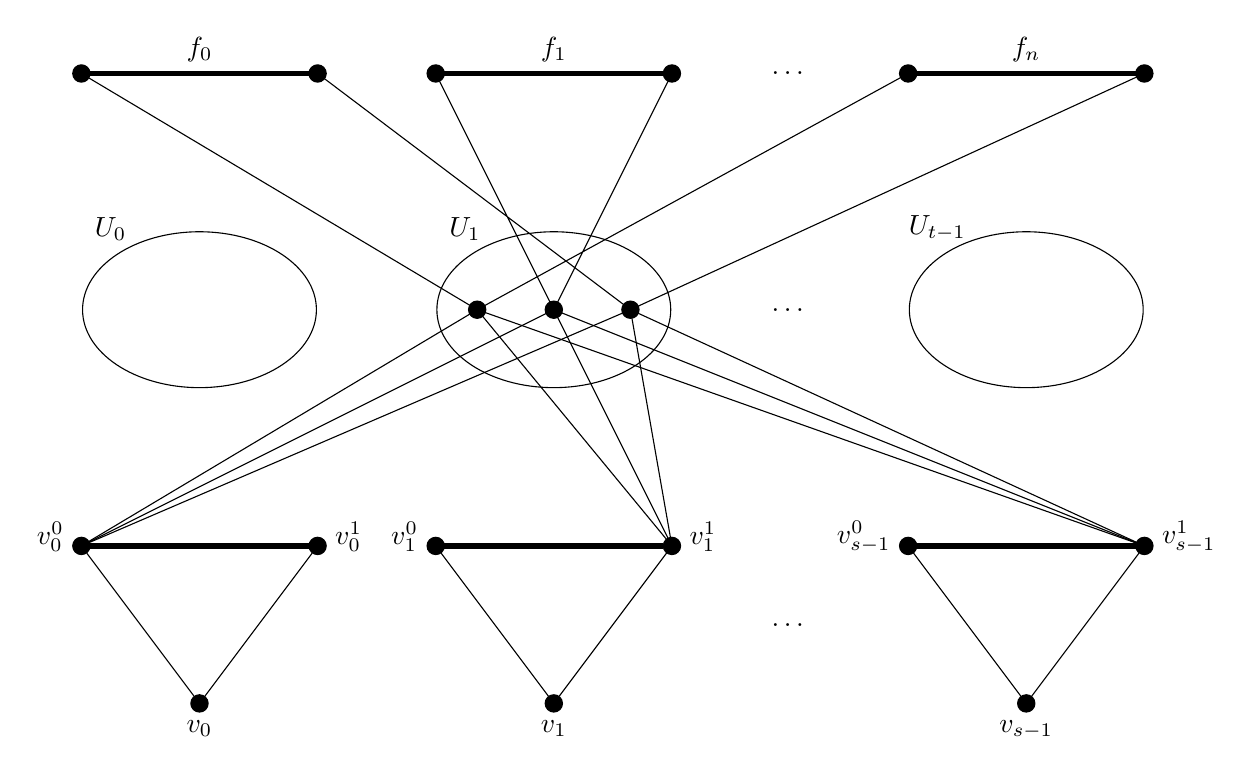
\begin{tikzpicture}
	
		\tikzset{nodestyle/.style={draw,circle,fill=black,minimum size=25pt, scale=0.25}}
		\tikzset{dotstyle/.style={draw,circle,fill=black, minimum size=5pt, scale=0.25}}
		\tikzset{forcededge/.style={-,line width=2pt}}
		\tikzset{graphstyle/.style={draw, inner sep=0pt,fit={(0,0) (2.1,1.4)}}}
		
		\tikzset{freedge/.style={-}}
		
		\newcommand\makeDots[2]
		{
			\node at ($(#1)!.5!(#2)$) {\ldots};
		}
		
		\newcommand\edgeSize{3}
		\newcommand\gadgetHeight{2}
		\newcommand\textSpacingV{0.1}
		\newcommand\textSpacingH{0.2}
		\newcommand\spacing{1.5}
		
		\newcommand{\gadget}[2]{
			\node[
			nodestyle,
			label={[below=\textSpacingH]:$v_{#2}$}
			] at (#1+\edgeSize/2,0) (g#2) {};
			\node[
			nodestyle,
			label={[left=\textSpacingV]:$v^0_{#2}$}
			] at (#1,\gadgetHeight) (g#20) {};
			\node[
			nodestyle,
			label={[right=\textSpacingV]:$v^1_{#2}$}
			] at (#1+\edgeSize,\gadgetHeight) (g#21) {};
			\draw[forcededge] (g#20) to (g#21);
			\draw[freedge] 
			(g#20) to (g#2) 
			(g#21) to (g#2);
			
			\node at (#1+\edgeSize/2,\gadgetHeight/2) (g#2center) {};
		}
		
		\newcommand\drawGadget
		{
			\gadget{0}{0}
			\gadget{\edgeSize+\spacing}{1}
			\gadget{2*\edgeSize+3*\spacing}{s-1}
			\node at ($(g1center)!.5!(gs-1center)$) {\ldots};	
		}
		
		\newcommand\forcedEdge[3] % {name}{width}{height}
		{
			\node[nodestyle] at (#2, #3) (f#11) {};
			\node[nodestyle] at (#2+\edgeSize, #3) (f#12) {};
			\draw[forcededge] (f#11) -- (f#12) node[above,midway] {$f_{#1}$};	
		}
		\newcommand\drawForcedSet[1]
		{
			\forcedEdge{0}{0}{#1}
			\forcedEdge{1}{\edgeSize+\spacing}{#1}
			\forcedEdge{n}{2*\edgeSize+3*\spacing}{#1}
			\makeDots{f12}{fn1}
		}	
		
		\newcommand\drawFreeVertices[1]
		{
			\node[
			graphstyle, 
			label={[anchor=south,above=0.1cm]150:$U_0$},
			ellipse] at (1.5,#1) (U1) {};	
			\node[
			graphstyle, 
			ellipse,
			label={[anchor=south,above=0.1cm]150:$U_1$}
			] at (1.5+\edgeSize+\spacing,#1) (U2) {};	
			\node[
			graphstyle,
			label={[anchor=south,above=0.1cm]150:$U_{t-1}$},
			ellipse
			] at (1.5+2*\edgeSize+3*\spacing,#1) (Un) {};
			\node[nodestyle] at (U2) (v2) {};
			\node[nodestyle, left=\edgeSize/4 of v2] (v1) {};
			\node[nodestyle, right=\edgeSize/4 of v2] (v3) {};
			\makeDots{U2}{Un}
		}
		
		\drawGadget{0}
		\drawForcedSet{8}
		\drawFreeVertices{5}
		
		\foreach \x in {1,...,3}
		{
			\draw[-]
			(g00) to (v\x)
			(g11) to (v\x)
			(gs-11) to (v\x);	
		}
		
		\draw[-]
		(v1) to (f01)
		(v3) to (f02)
		(v2) to (f11)
		(v2) to (f12)
		(v3) to (fn2)
		(v1) to (fn1);
	\end{tikzpicture}
	\caption{Construction of the composed instance $(G,F)$. Bold edges are forced.}
	\label{fig1}
\end{figure}


Immediately, by Theorem \ref{nokernel} and Lemma \ref{cross-ssfe} we obtain the following:

\thmssfepnokernel*

\section{Parametrization by the number of free vertices}

In this section, we parameterize  \ssfep{} by the number of free vertices. We begin with an algorithm that solves the problem in time $\mathcal{O}^*(1.358^k)$ where $k$ is the number of free vertices. Then, unlike in the first variant, we present a kernelization algorithm. We show that the reduced instance has at most $3k$ vertices where $k$ is the parameter.

\subsection{Algorithm}
We start with stating a result for the \cnfsat{} problem parameterized by the number of clauses proven by Bliznets and Golovnev. \cite{MAXSAT}

\begin{theorem}\label{cnfsatmtime}
	\cnfsat{} can be solved in time $\mathcal{O}^*(1.358^k)$ where $k$ is the number of clauses.
\end{theorem}

Now, observe that \cnfsat{} parameterized by the number of clauses and \ssfep{} parameterized by the number of free vertices are interreducible with respect to polynomial reductions. Thus, we are ready to show an algorithm.

\thmssfepfreealg*

\begin{proof}
	Let $(G,F)$ be an arbitrary instance of \ssfep{} parameterized by the number of free vertices. Firstly, we apply Lemma \ref{norm-ssfe}. If the lemma yields that the instance is a NO-instance, then we conclude. Otherwise, let $(G',F')$ be the normalized instance. We apply Lemma \ref{cnfsat reduction} and obtain an equivalent formula $\phi$. Observe that $\phi$ has at most $|F|$ variables and at most $|U|$ clauses. Now, by Theorem \ref{cnfsatmtime} we can apply an algorithm that decides whether $\phi$ is satisfiable or not in time $\mathcal{O}^*(1.358^{|U|})$.
\end{proof}

\subsection{Kernelization}

This subsection is inspired by the kernelization algorithm for the {\sc Maximum Satisfiability} problem shown by Lokshtanov in \cite{MAXSATKERNEL}. In the {\sc Maximum Satisfiability} problem, given a formula $\phi$ and an integer $k$ we ask whether there exists an evaluation $\sigma$ such that at least $k$ clauses are satisfied in $\phi$. Lokshtanov shows an algorithm that outputs an equivalent instance with at most $k$ variables and at most $2k$ clauses. For \ssfep{} parameterized by the number of free vertices we show a kernelization algorithm that outputs an equivalent instance with at most $k$ free vertices and at most $k$ forced edges, where $k$ is the parameter.

At first we introduce a definition of a crown decomposition proposed by Chor et al. \cite{Crown}. Recall that for disjoint sets $X,Y \subseteq V(G)$, a \textit{matching of $X$ into $Y$} is a matching $M$ such that every edge has one endpoint in $X$ and one endpoint in $Y$, and for every $x \in X$ there exists exactly one edge $xy \in M$ such that $y \in Y$.

\begin{definition}
	A \textit{crown decomposition} of a graph $G$ is a partitioning of $V(G)$ into three parts $C,H$ and $R$, such that:
	\begin{itemize}
		\item $C$ is nonempty.
		\item $C$ is an independent set.
		\item There are no edges between $C$ and $H$. That is, $H$ separates $C$ from $R$.
		\item Let $E'$ be the set of edges between $C$ and $H$. Then, $E'$ contains a matching of size $|H|$. In other words, $G$ contains a matching of $H$ into $C$.
	\end{itemize}
\end{definition}

An essential tool in our kernelization is Hopcroft-Karp's algorithm \cite{Hopcroft-Karp}.

\begin{theorem}[\textbf{Hopcroft-Karp algorithm}]
	Let G be an undirected bipartite graph with bipartition $(V_1,V_2)$, on $n$ vertices and $m$ edges.	Then, we can find a maximum matching as well as a minimum vertex cover of $G$ in time $\mathcal{O}(m\sqrt{n})$. Furthermore, in time $\mathcal{O}(m\sqrt{n})$ either we can find a matching of $V_1$ into $V_2$ or an inclusion-wise minimal set $X \subseteq V_1$ such that $|N(X)| < |X|$.
\end{theorem}

Finally, equipped with the above information, we are ready to show a linear kernel for \ssfep{}  parameterized by the number of free vertices.

\begin{lemma}\label{kernel-ssfep}
	There exists a polynomial-time algorithm, that, given an instance $(G,F)$ such that $|F| \geq |U|$, either
	\begin{itemize}
		\item answers that $(G,F)$ is a YES-instance, or
		\item outputs an equivalent instance $(G',F')$ such that $|U'| \leq |U|$ and $|F'| < |F|$ where $U'$ is the set of free vertices in $(G',F')$.
	\end{itemize} 
\end{lemma}


\begin{proof}
	By Lemma \ref{norm-ssfe}, we assume that $(G,F)$ is a normalized instance. Let $G_{F,U}$ be the bipartite graph formed from $(G,F)$ by contracting forced edges. A vertex obtained by contracting edge $e$ is named $e$ as well, thus the sides of bipartion are $F$ and $U$. We apply Hopcroft-Karp's algorithm to $G_{F,U}$. We either obtain a matching $M$ of $F$ into $U$ or an inclusion-wise minimal set $X \subseteq F$ such that $|N_{G_{F,U}}(X)| < |X|$.

	Consider the first case in which Hoprocft-Karp's algorithm returns a matching. Then, we conclude that $(G,F)$ is a YES-instance due to the following claim:
	\begin{claim}
		Assume $(G,F)$ is a normalized instance of \ssfep{} where $|F| \geq |U|$. If Hoprocft-Karp's algorithm ran on $G_{F,U}$ returns a matching $M$ of $F$ into $U$, then $(G,F)$ is a YES-instance.
	\end{claim}

	\begin{proof}
		Since $M$ is a matching of $F$ into $U$, then we infer that $|F| \leq |U|$. Furthermore, we assumed that in $(G,F)$, $|F| \geq |U|$. Thus, $|F|=|U|$ and $M$ is also a matching of $U$ into $F$. Now, we claim that there exists a spanning star forest for $(G,F)$. Indeed, let $M' \subseteq E(G)$ be a matching such that if we contract forced edges adjacent to $M$, then $M'$ becomes $M$. So, $S = M' \cup F$ is a spanning star forest for $G$ as every free vertex is spanned by $M'$.
	\end{proof}

	Now, consider the second case. Let $X \subseteq F$ be an inclusion-wise minimal set such that $|N_{G_{F,U}}(X)| < |X|$. Let $C=X$, $H=N_{G_{F,U}}(X)$ and $R= V(G_{F,U}) \setminus (H \cup C)$. Now, we claim that:
	\begin{claim}
		$(C,H,R)$ is a crown decomposition of $G_{F,U}$.
	\end{claim}
	\begin{proof}
		Observe that $C$ is nonempty and $C$ is an independent set as $F$ is an induced matching in $G$. Moreover, $H$ separates $C$ from $R$ because $H$ is the set of all the neighbors of $C$. Now, we prove that there exists a matching of $H$ into $C$. Select an arbitrary $v \in C$. There is a matching of $C \setminus \{v\}$ into $H$ since $|N_{G_{F,U}}(C')| \geq |C|$ for every $C' \subsetneq C$. Since $|C| > |H|$, we have that the matching of $C \setminus \{v\}$ into $H$ is actually a matching of $H$ into $C$. Therefore, $(C,H,R)$ is a crown decomposition of $G_{F,U}$.
	\end{proof}

	We proceed to the construction of a reduced instance. Let $(C,H,R)$ be the crown decomposition of $G_{F,U}$ described above. Let $D_F \subseteq F$ be the set of forced edges such that if we contract them, then $D_F$ becomes $C$. Finally, let $(G',F')$ be an instance formed from $(G,F)$ by removing vertices $D=V(D_F) \cup H$. We claim that the operation is safe.
	
	\begin{claim}
		$(G,F)$ has a spanning star forest if and only if $(G',F')$ has a spanning star forest.
	\end{claim}
	\begin{proof}		
		Let $S$ be a solution for $(G,F)$. We claim that $S' = S[V(G')]$, that is, $S$ restricted to the vertices of the graph $G'$, is a spanning star forest for $(G',F')$. Suppose there exists and edge $vu \in S$ such that $v \in D$ and $v \notin D$. Observe that $N_G[V(D_F)] = H \cup V(D_F)$ by the choice of sets for a crown decomposition. Hence, $v \in H$ and $u \in V(F) \setminus V(D_F)$. Since $u$ is adjacent to a forced edge, we have that $u$ is not isolated in $S'$. We conclude that $S'$ is a spanning star forest for $(G',F')$.
		
		For the backward implication, let $S$ be a solution for $(G',F')$. Recall that by $D_F$ we denoted the set of forced edges such that if we contract the edges, then $D_F$ becomes $C$. By the definition of a crown decomposition, there exists a matching of $H$ into $C$, say $M'$. Therefore, let $M$ be a matching between $V(D_F)$ and $H$ in $G$ such that if we contract forced edges adjacent to $M$, then $M$ becomes $M'$ in $G_{F,U}$. Observe that now $S \cup M$ is a spanning star forest for $(G,F)$.
	\end{proof}
	
	Observe that a crown decomposition requires that $C$ is nonempty. Thus, $|F'| < |F|$ which concludes the proof. \qedhere
	
\end{proof}

The lemma immediately proves the following theorem:

\thmssfepkernel*

\begin{proof}
	Exhaustive application of Lemma \ref{kernel-ssfep} on a normalized instance $(G,F)$ either outputs that the instance is a YES-instance, or outputs an equivalent instance $(G',F')$ such that $|F'| \leq |U'|$ and $|U'| \leq |U|$.
\end{proof}

\section{Parametrization by treewidth}

In this section, we parameterize the problem by the treewidth of the input graph. As an input, we receive a tuple $(G,F,\mathcal{T})$ where $\mathcal{T}$ is a tree decomposition of $G$. We present a dynamic programming algorithm that works on a given tree decomposition. Later, we prove a lower bound of the running time based on a reduction from the \cnfsat{} problem. Note that we may assume that $(G,F)$ is a normalized instance due to Lemma \ref{norm-ssfe}.

\subsection{Preliminaries}

We extend the notation of tree decomposition. Namely, for introduce vertex node, we distinguish \textit{introduce free vertex node} and \textit{introduce forced vertex node}. Similarly, we extend the definition for introduce edge and forget vertex node. Recall that a tree decomposition $\mathcal{T}$ of a graph $G$ consists of a tree $T$, and for every node $t \in T$ there exists a set $X_t \subseteq V(G)$. Every entry of a dynamic table $\text{dp}$ has three parameters: a tree decomposition node $t$ and two assignment functions $f,g$. An \textit{assignment function for forced vertices} $f: (X_t \cap V(F)) \rightarrow \{\true, \false\}$ is a mapping that distinguishes two states. If $f(v)=\true$, then we say that $v$ is a center whereas, if $f(v)=\false$, then $v$ is either a candidate or a ray. An \textit{assignment function for free vertices} $g: (X_t \cap U) \rightarrow \{\true, \false\}$ is a mapping that indicates whether a free vertex has been added to a star or not. Hence, for a free vertex $v$ we say that $v$ is in a star if $f(v)=\true$ and, if it is not, then $f(v)=\false$.

For the sake of clarity, we introduce the following notation. Suppose $(G,F,\mathcal{T})$ is an input instance. Let $(t,X_t) \in \mathcal{T}$ be a node and the corresponding set of vertices in a tree decomposition. By $G_t$ we define a subgraph of $G$ such that $V(G_t) = X_t$ and $G_t$ has edges that have been introduced in the subtree rooted in $t$. Let $\mathcal{F}_t = \{(X_t \cap V(F)) \rightarrow \{\false,\true\}\}$ be the family of all assignment functions for forced vertices from $X_t$ and let $\mathcal{G}_t = \{(X_t \setminus V(F)) \rightarrow \{\false,\true\}\}$ be the family of all assignment functions for free vertices from $X_t$. For any assignment function $h$ and $X' \subseteq X$, where $X$ is the domain of $h$, we use $h|_{X'}$ to denote the restriction of $h$ to $X'$. For a subset $X \subseteq V(G)$ consider an assignment function $h$. For a vertex $v \in V(G)$ and a logic value $p \in \{\true, \false\}$ we define a new assignment $h_{v \rightarrow p}: X \cup \{v\} \rightarrow \{\true, \false\}$ as follows:

\begin{equation*}
	h_{v \rightarrow p}(u) =
	\begin{cases}
	\begin{aligned}
		&h(u), & \text{if $u \neq v$} \\
		&p, &\text{if $u = v$}
	\end{aligned}
	\end{cases}
\end{equation*}

\subsection{Algorithm}

We provide formulas for every type of a node. To call an entry from a dynamic table we provide three arguments. The first one is a node $t$ from a tree decomposition. The second one is a forced vertices assignment $f \in \mathcal{F}_t$. The last one is  a free vertices assignment $g \in \mathcal{G}_t$. Then, we shall compute a Boolean value $\dpt{t,f,g}$ equal to whether in $G_t$ there exists an independent set $C \subseteq V(F)$ such that
\begin{itemize}
	\item $C \cap X_t = f^{-1}(\true)$, and
	\item $g^{-1}(\true) \subseteq N_{G_t}(C)$.
\end{itemize}

Observe that the existence of such an independent set for $t$ being the root is equivalent to the existence of a spanning star forest due to Lemma \ref{span-lemma}.

\paragraph{Leaf node} For a leaf node $t$ we have that $X_t=\emptyset$. An empty graph is a spanning star forest. Hence:

\begin{equation*}
	\dpt{t,\emptyset,\emptyset}=\true
\end{equation*}

\paragraph{Introduce forced vertex node} Let $t$ be an introduce node with a child $t'$ such that $X_t = X_{t'} \cup \{v\}$ and $v \in V(F)$. Observe that $v$ is isolated in $G_t$. Thus, we pass the value from the child node:

\begin{equation*}
	\dpt{t,f,g}= \dpt{t',f|_{X_{t'}},g}
\end{equation*}

\paragraph{Introduce free vertex node} Let $t$ be an introduce free vertex node with a child $t'$ such that $X_t = X_{t'} \cup \{v\}$. Note that $\dpt{t,f,g}=\false$ if $g(v)=\true$ as $v$ is isolated in $G_t$. Thus, we obtain the following:

\begin{equation*}
	\dpt{t,f,g} =
	\begin{cases}
		\dpt{t',f,g|_{X_{t'}}}, & \text{if $g(v)=\false$} \\
		\false, &\text{otherwise}
	\end{cases}
\end{equation*}

\paragraph{Introduce free edge node} Let $t$ be an introduce free edge node labeled with an edge $vu \in E(G) \setminus F$ and let $t'$ be the child of $t$. Recall that $G$ is a normalized instance. Without loss of generality, assume that $v \in U$ and $u \in V(F)$ as every free edge has one end in a free vertex and the other one in a forced vertex. Let $f \in \mathcal{F}_t$ and $g \in \mathcal{G}_t$. Suppose that $g(v)=\false$. Then, we simply pass the value from the child's node. Otherwise, $g(v)=\true$. We need to find a vertex $u' \in V(F) \cap X_t$ such that $f(u')=\true$ and $v$ is a neighbor of $u'$ in $G_t$. It can be $u$ if $f(u)=\true$ or some other forced vertex for which we have already introduced the edge $vu'$. Thus, we obtain the following equations:

\begin{equation*}
	\dpt{t,f,g} = 
		\begin{cases}
			\dpt{t',f,g} \lor \dpt{t',f,g_{v \rightarrow \false}}, & \text{if $f(u)=\true$ and $g(v)=\true$} \\
			\dpt{t',f,g}, & \text{otherwise}
		\end{cases}	
\end{equation*}

\paragraph{Introduce forced edge node} Let $t$ be an introduce free edge node labeled with an edge $vu \in F$, $t'$ be the child of $t$ and let $f \in \mathcal{F}_t$. Calculations for $t$ are simple. We set to $\false$ all the elements of dynamic table for which $f(v)=f(u)=\true$:

\begin{equation*}
	\dpt{t,f,g} =
	\begin{cases}
		\dpt{t',f,g}, & \text{if $f(v)=\false$ or $f(u)=\false$} \\
		\false, & \text{otherwise}
	\end{cases}
\end{equation*}

\paragraph{Forget forced vertex node} Let $t$ be an forget forced vertex node with a child $t'$, such that $X_t = X_{t'} \setminus \{v\}$ and let $u \in V(F)$ such that $vu \in F$. Observe that for any $f \in \mathcal{F}_t$ that satisfies $f(v)=f(u)=\true$, $\dpt{t',f,g} = \false$ because we have already changed their values during introduce forced edge node. Thus, the formula looks as follows:

\begin{equation*}
	\dpt{t,f,g} = \dpt{t',f_{v \rightarrow \true},g} \lor \dpt{t',f_{v \rightarrow \false},g}
\end{equation*}

\paragraph{Forget free vertex node} Let $t$ be a forget free vertex node with a child $t'$ such that $X_t = X_{t'} \setminus \{v\}$ where $v \in U$. We can pass the value from a child node if and only if $v$ was added to a star, that is, for a $g \in \mathcal{G_t}$, $g(v)=\true$. Consequently, we obtain:

\begin{equation*}
	\dpt{t,f,g} = \dpt{t',f,g_{v \rightarrow \true}}
\end{equation*}

\paragraph{Join node} Let $t$ be a join node with children $t_1$ and $t_2$. Recall that $X_t=X_{t_1}=X_{t_2}$. We say that assignment functions $f_1,g_1$ of $X_{t_1}$ and $f_2,g_2$ of $X_{t_2}$ \textit{match} with assignments $f,g$ of $X_t$ if the following conditions hold:

\begin{enumerate}
	\item For every forced vertex $v \in X_t \cap V(F)$, $f(v)=f_1(v)=f_2(v)$.
	\item For every free vertex $v \in X_t \cap U$, $g(v)=g_1(v) \lor g_2(u)$.
\end{enumerate}
Hence, we get:

\begin{equation*}
	\dpt{t,f,g} =
		\bigvee\limits_{g_1,g_2 \text{ match $g$}} dp[t_1,f,g_1] \land dp[t_2,f,g_2]
\end{equation*}

\subsection{Complexity analysis}

Now we proceed to the complexity analysis. Observe that each of the introduce and forget nodes can be computed in constant time. We either copy a specific value from a child's node or perform a logical OR operation of two boolean values. 

Computing a join node is the bottleneck in this algorithm. A naive approach to obtain the value for a single join node entry would result in time $\mathcal{O}^(4^{\tw(G)})$. Thus, we could conclude with an algorithm solving \ssfep{} parameterized by treewidth in time $\mathcal{O}^*(8^{\tw(G)})$ as there are $\mathcal{O}(|G| \cdot 2^{\tw(G)})$ array entries. However, we can improve the running time using fast computation of the \textit{cover product}.

\begin{definition}
	The \textit{cover product} of two functions $f,g:2^V \rightarrow \mathbb{Z}$ is a function $(f *_c g):2^V \rightarrow \mathbb{Z}$ such that for every $Y \subseteq V$:
	
	\begin{equation*}
		(f *_c g)(Y) = \sum\limits_{ A \cup B = Y} f(A)g(B)
	\end{equation*}
\end{definition}

Now, we state the theorem proved by Björklund et al. \cite{CoverProduct}:

\begin{theorem}\label{cproduct}
	For two functions $f,g:2^V \rightarrow \mathbb{Z}$ with $|V|=n$, given all $2^n$ values of $f$ and $g$ in the input, all the $2^n$ values of the cover product $f*_cg$ can be computed using $\mathcal{O}(2^n\cdot n)$ arithmetic operations.
\end{theorem}

Note that the disjunction in every join node is nothing else than a cover product for a fixed forced vertices assignment. Thus, we formulate the lemma:

\begin{lemma}\label{join lemma}
	Given a join node $t$, one can calculate all values of $\dpt{t,f,g}$, for $f \in \mathcal{F}_t$ and $g \in \mathcal{G}_t$, in time $O(2^w)$ where $w$ is the width of the decomposition.
\end{lemma}

\begin{proof}
	Fix $f \in \mathcal{F}_t$. We define a function $c_{t,f}:2^{X_t \cap U} \rightarrow \mathbb{Z}$ as follows:
	
	\begin{equation*}
		c_{t,f}(X) = dp[t,f,g] \text{, such that $g^{-1}(\true) = X$}.
	\end{equation*}	
	Note that the function $c_{t,f}$ should output an integer, not a Boolean value. Thus, we map $\true$ to $1$ and $\false$ to $0$. Now, for $X \subseteq X_t \cap U$, observe that: 
	\begin{align*}
		(c_{t_1,f} *_c c_{t_2,f})(X) &= \sum\limits_{A \cup B = X} c_{t_1,f}(A)c_{t_2,f}(B) \\
		&= \sum\limits_{ g_1^{-1}(\true)\ \cup\ g_2^{-1}(\true) = X} dp[t_1,f,g_1]dp[t_2,f,g_2]	
	\end{align*}
	which exactly reflects the computation that we perform during a join node. Thus, $\dpt{t,f,g} = \true$ if $(c_{t_1,f} *_c c_{t_2,f})(g^{-1}(1)) > 0$ and $\dpt{t,f,g} = \false$ otherwise. 
	
	Observe that $|\mathcal{F}_t| = 2^{|X_t \cap V(F)|}$. By Theorem \ref{cproduct}, for a fixed $f \in \mathcal{F}_t$ and every $g \in \mathcal{G}_t$ we can calculate values of $\dpt{t,f,g}$ in time $2^{|X_t \cap U|}$. Thus, we can fill all the entries corresponding to the node $t$ in time $\mathcal{O}^*(2^{|X_t \cap V(F)|} \cdot 2^{|X_t \cap U|}) = \mathcal{O}^*(2^{|X_t|}) \leq \mathcal{O}^*(2^w)$.
\end{proof}

\thmssfeptwtime*

\begin{proof}
	Consider the algorithm described in the previous subsection. To calculate a single entry for introduce and forget nodes we need constant time. By Lemma \ref{join lemma}, we showed that the values for a join node can be calculated in $\mathcal{O}^*(2^w)$. There are polynomially many nodes in a tree decomposition. Thus, we can fill the entries of a dynamic table in time $\mathcal{O}^*(2^{w})$ and provide the answer whether the input graph has a \ssf{}.
\end{proof}

\subsection{Lower bound on a running time}

We have just proven the complexity of the algorithm stated in the previous subsection. Now, we show a matching lower bound for the problem based on the \cnfsat{} problem. The construction shown below was inspired by \cite{TREEWIDTH}.

\thmssfeptwseth*

\begin{figure}
\end{figure}

\begin{proof}
	We provide a polynomial-time reduction that takes a \cnfsat{} instance $\phi$ with $n$ variables and $m$ clauses, and constructs an instance $(G,F)$ together with a tree decomposition of width $n$. If there existed an algorithm solving \ssfep{} parameterized by the width of a given tree decomposition in time  $\mathcal{O}^*((2-\epsilon)^n)$, then we could compose the reduction with this algorithm and solve \cnfsat{} in time  $\mathcal{O}^*((2-\epsilon)^n)$.
	
	We first give a brief overview of how the output graph looks like and provide a notation for referring to specific vertices. The output instance $(G,F)$ consists of $n+1$ copies of the \textit{formula graph}, denoted as $G_1,G_2,...,G_{n+1}$. Every formula graph $G_i$ consists of $m$ \textit{clause graphs} $C^i_1,C^i_2,...,C^i_m$. Every two consecutive clause graphs, whether or not from the same copy of $G$, are connected by a connection gadget $H^i_1,H^i_2,...,H^i_m$. For example, connection gadget $H^i_k$, for $i < n+1$ and $k < m$ connects clause graph $C^i_k$ and $C^i_{k+1}$ whereas connection gadget $H^i_m$ connects clause graph $C^i_m$ and $C^{i+1}_1$. By $v^i_j$ we refer to vertices in $j$-th clause graphs from $i$-th formula graph and by $g^i_j$ we refer to vertices in $j$-th connection gadget $i$-th formula graph.
	
	After the brief introduction, we present the construction of a clause graph $C^i_j$. We introduce a free vertex $v^i_j[c]$ and $n$ forced edges $v^i_j[x_k]v^i_j[\neg x_k]$. For every literal $l$ occurring in the clause $c_i$, we introduce an edge $v^i_j[l]v^i_j[c]$. Observe that every clause graph consists of $2n+1$ vertices and $n$ forced edges.
	
	Now, we present the construction of a connection gadget $H^i_j$. Firstly, we introduce $n$ free vertices $g^i_j[1],g^i_j[2],...,g^i_j[n]$. If $j < m$, then for every $g^i_j[k]$ we introduce edges $v^i_j[\neg x_k]g^i_j[k]$ and $g^i_j[k]v^i_{j+1}[x_k]$. Otherwise, if $j=m$, then we introduce edges $v^i_m[\neg x_k]g^i_m[k]$ and $g^i_m[k]v^{i+1}_1[x_k]$. Note that there does not exist a connection gadget $H^{n+1}_m$ as $C^{n+1}_m$ is the last clause gadget.
	
	
	Intuitively, there are $(n+1)\cdot m$ clause graph $C^1_1,C^1_2,\ldots,C^1_m,C^2_1,\ldots,C^{n+1}_m$. Every clause graph has one free vertex and a set of $n$ forced edges. Every two consecutive sets of forced edges in clause graphs are joined by a connection gadget. See Figure \ref{fig2}.
	
	\begin{figure}
		\centering
		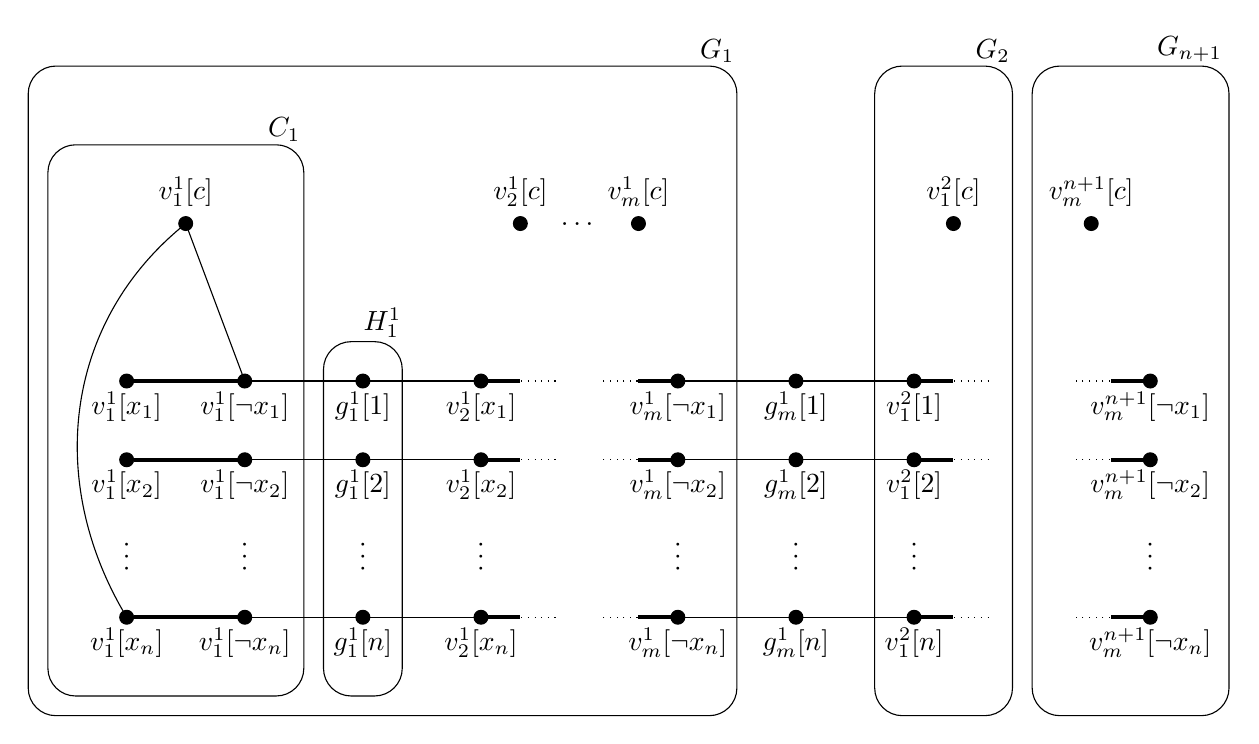
\begin{tikzpicture}
		\tikzset{nodestyle/.style={draw,circle,fill=black,minimum size=20pt, scale=0.25}}
		\tikzset{forcededge/.style={-,line width=1.5pt}}
		
		%\draw[help lines, blue] (0,0) grid (15,10);
		
		\newcommand\edgeSize{1.5}
		\newcommand\spacing{1}
		
		\newcommand\drawNode[4] % {width} {height} {label} {name}
		{
			\node[
			nodestyle,
			label={[below=0.1cm]:#3}
			] at (#1, #2) (#4) {};
		}
		
		\newcommand\drawClauseNode[4] % {width} {height} {label} {name}
		{
			\node[
			nodestyle,
			label={[above]:#3}
			] at (#1, #2) (#4) {};
		}
		
		\newcommand\frontPadding{1}
		
		\drawNode{1}{1}{$v^1_1[x_n]$}{x11n1}
		\drawNode{1}{3}{$v^1_1[x_2]$}{x1121}
		\drawNode{1}{4}{$v^1_1[x_1]$}{x1111}
		
		\drawNode{2.5}{1}{$v^1_1[\neg x_n]$}{x11n0}
		\drawNode{2.5}{3}{$v^1_1[\neg x_2]$}{x1120}
		\drawNode{2.5}{4}{$v^1_1[\neg x_1]$}{x1110}
		
		\drawClauseNode{1.75}{6}{$v^1_1[c]$}{c11}
		
		\draw[forcededge] 
		(x11n1) to (x11n0)
		(x1121) to (x1120)
		(x1111) to (x1110);
		
		\draw[]
		(x1110) to (c11)
		(x11n1) to[out=120, in=220] (c11);
		
		\drawNode{4}{1}{$g^1_1[n]$}{g11n}
		\drawNode{4}{3}{$g^1_1[2]$}{g112}
		\drawNode{4}{4}{$g^1_1[1]$}{g111}
		
		\drawNode{5.5}{1}{$v^1_2[x_n]$}{x12n}
		\drawNode{5.5}{3}{$v^1_2[x_2]$}{x122}
		\drawNode{5.5}{4}{$v^1_2[x_1]$}{x121}
		
		\draw[]
		(x11n0) to (g11n)
		(x1120) to (g112)
		(x1110) to (g111)
		(g11n) to (x12n)
		(g112) to (x122)
		(g111) to (x121);
		
		\draw[forcededge]
		(x12n) to ($(x12n) + (0.5,0)$)			
		(x122) to ($(x122) + (0.5,0)$)
		(x121) to ($(x121) + (0.5,0)$);
		
		\draw[dotted]
		(x12n) to ($(x12n) + (1,0)$)			
		(x122) to ($(x122) + (1,0)$)
		(x121) to ($(x121) + (1,0)$);
		
		\drawNode{8}{1}{$v^1_m[\neg x_n]$}{x1mn}
		\drawNode{8}{3}{$v^1_m[\neg x_2]$}{x1m2}
		\drawNode{8}{4}{$v^1_m[\neg x_1]$}{x1m1}
		
		\drawNode{9.5}{1}{$g^1_m[n]$}{g1mn}
		\drawNode{9.5}{3}{$g^1_m[2]$}{g1m2}
		\drawNode{9.5}{4}{$g^1_m[1]$}{g1m1}
		
		\draw[forcededge]
		(x1mn) to ($(x1mn) - (0.5,0)$)			
		(x1m2) to ($(x1m2) - (0.5,0)$)
		(x1m1) to ($(x1m1) - (0.5,0)$);
		
		\draw[dotted]
		(x1mn) to ($(x1mn) - (1,0)$)			
		(x1m2) to ($(x1m2) - (1,0)$)
		(x1m1) to ($(x1m1) - (1,0)$);
		
		\draw[]
		(x1mn) to (g1mn)
		(x1m2) to (g1m2)
		(x1m1) to (g1m1);
		
		
		\drawNode{11}{1}{$v^2_1[n]$}{v21n}
		\drawNode{11}{3}{$v^2_1[2]$}{v212}
		\drawNode{11}{4}{$v^2_1[1]$}{v211}
		
		\drawNode{14}{1}{$v^{n+1}_m[\neg x_n]$}{xn1mn}
		\drawNode{14}{3}{$v^{n+1}_m[\neg x_2]$}{xn1m2}
		\drawNode{14}{4}{$v^{n+1}_m[\neg x_1]$}{xn1m1}
		
		\draw[]
		(g1mn) to (v21n)
		(g1m2) to (v212)
		(g1m1) to (v211);
		
		\draw[forcededge]
		(xn1mn) to ($(xn1mn) - (0.5,0)$)			
		(xn1m2) to ($(xn1m2) - (0.5,0)$)
		(xn1m1) to ($(xn1m1) - (0.5,0)$);
		
		\draw[dotted]
		(xn1mn) to ($(xn1mn) - (1,0)$)			
		(xn1m2) to ($(xn1m2) - (1,0)$)
		(xn1m1) to ($(xn1m1) - (1,0)$);
		
		\draw[forcededge]
		(v21n) to ($(v21n) + (0.5,0)$)			
		(v212) to ($(v212) + (0.5,0)$)
		(v211) to ($(v211) + (0.5,0)$);
		
		\draw[dotted]
		(v21n) to ($(v21n) + (1,0)$)			
		(v212) to ($(v212) + (1,0)$)
		(v211) to ($(v211) + (1,0)$);
		
		\draw[rounded corners=10pt] (0,0) rectangle (3.25,7);
		\node[label={:$C_1$}] at (3,6.8) {};
		\draw[rounded corners=10pt] (3.5,0) rectangle (4.5,4.5);
		\node[label={:$H^1_1$}] at (4.25,4.3) {};
		\draw[rounded corners=10pt] (-0.25,-0.25) rectangle (8.75,8);
		\node[label={:$G_1$}] at (8.5,7.8) {};
		\draw[rounded corners=10pt] (10.5, -0.25) rectangle (12.25,8);
		\node[label={:$G_2$}] at (12,7.8) {};
		\draw[rounded corners=10pt] (12.5, -0.25) rectangle (15,8); 
		\node[label={:$G_{n+1}$}] at (14.5,7.8) {};
		
		\node[rotate=90] at ($(x1121)!.6!(x11n1)$) {\ldots};
		\node[rotate=90] at ($(x1120)!.6!(x11n0)$) {\ldots};
		\node[rotate=90] at ($(g112)!.6!(g11n)$) {\ldots};
		\node[rotate=90] at ($(x122)!.6!(x12n)$) {\ldots};
		\node[rotate=90] at ($(x1m2)!.6!(x1mn)$) {\ldots};
		\node[rotate=90] at ($(g1m2)!.6!(g1mn)$) {\ldots};
		\node[rotate=90] at ($(v212)!.6!(v21n)$) {\ldots};
		\node[rotate=90] at ($(xn1m2)!.6!(xn1mn)$) {\ldots};
		
		\drawClauseNode{6}{6}{$v^1_2[c]$}{c12}
		\drawClauseNode{7.5}{6}{$v^1_m[c]$}{c1m}
		\node[] at ($(c12)!.5!(c1m)$) {\ldots};
		
		\drawClauseNode{11.5}{6}{$v^2_1[c]$}{c21}
		
		\drawClauseNode{13.25}{6}{$v^{n+1}_m[c]$}{cn1m}
		
		\end{tikzpicture}
		\caption{Construction of an instance $(G,F)$ from a formula. Bold edges are forced.}
		\label{fig2}
	\end{figure}
	
	Let us discuss the specifications of the output graph. As every clause graph has $2n+1$ vertices and $n$ forced edges while every connection gadget has $n$ free vertices, we conclude that $|V(G)| = (n+1) \cdot m \cdot (3n+1) -n= \mathcal{O}(mn^2)$ and $|F|=(n+1) \cdot m \cdot n= \mathcal{O}(mn^2)$. Observe that $(G,F)$ is normalized as there are no isolated vertices, every clause vertex and every gadget vertex is adjacent to forced vertices only and $F$ is an induced matching. Note the following claim:
	
	\begin{claim}
		The reduction outputs an instance $(G,F)$ such that $G$ has a tree decomposition of width $|F|=n$, computable in polynomial time.
	\end{claim}

	\begin{proof}
		We show how to construct such a tree decomposition. We begin with a bag $B_0=\{v^1_1[x_i]: 1 \leq i \leq n\}$. Observe that $|B_0|=n$. In the construction we show that every introduce bag is followed by a forget one. Hence the maximum size of the intermediate bag is equal to $n+1$ and thus the width of such a decomposition is equal to $n$. 
		
		Now, for every $v \in B_0$ that follows $v \notin N_G(v^1_1[c])$ we introduce $v^1_1[\neg x_i]$ and forget $v^1_1[x_i]$. Let $B_{\alpha_1}$ be the output bag. Observe that $|B_{\alpha_1}|=n$. Since every neighbor of $v^1_1[c]$ is in $B_{\alpha_1}$ we introduce and immediately forget the vertex $v^1_1[c]$. Then, for every $v^1_1[x_k] \in N_G(v^1_1[c])$ we introduce $v^1_1[\neg x_k]$ and forget $v^1_1[x_k]$. Observe that now the output bag $B_{\alpha_2}$ follows $B_{\alpha_2} = \{v^1_1[\neg x_i]: 1 \leq i \leq n\}$, $|B_{\alpha_2}|=n$. Finally, for every $v^1_1[\neg x_i] \in B_\beta$ we do the following operations: introduce vertex $g^1_1[i]$, forget vertex $v^1_1[x_i]$, introduce vertex $v^1_2[x_i]$ and forget vertex $g^1_1[i]$. Let $B_{\alpha_3}$ be the output graph. Observe that now $B_{\alpha_3} = \{v^1_2[x_i]: 1 \leq i \leq n\}$. Thus, by applying the schema repeatedly for every clause graph, we show that there exists a tree decomposition of width $n$. Observe that the construction uses only introduce and forget bags. Indeed, the tree decomposition described above can be computed in polynomial time.
	\end{proof}
	
	Finally, we show that $\phi$ is satisfiable if and only if $(G,F)$ has a spanning star forest. For the forward implication, let $\sigma$ be an evaluation such that $\sigma(\phi)=\true$. If $\sigma(\phi)=\textrm{True}$, then for every $C_i \in \textrm{Clauses}$ there exists a literal $l_i \in C_i$ such that $\sigma(l_i)=1$. Now, let $L = \{v^i_j[l]: \sigma(l)=1\text{, } 1 \leq i \leq n+1 \text{ and } 1 \leq j \leq m\}$. Clearly, $\{v^i_j[C_k]: C_k \in \textrm{Clauses} \text{, } 1 \leq i \leq n+1 \text{ and } 1 \leq j \leq m\} \subseteq N_G(L)$ because $\sigma$ satisfies the formula $\phi$. Moreover every $g^i_j[k]$ belongs to $N_G(L)$, as it is adjacent to vertices corresponding to both $k$-th literal and its negation. Moreover, observe that $L$ is an independent set in $G$ because for every forced edge $v^i_j[x_k]v^i_j[\neg x_k] \in F$ either $\sigma(x_i)=\false$ or $\sigma(\neg x_i)=\false$. Hence, by Lemma \ref{span-lemma}, there exists a spanning star forest for $(G,F)$.
	
	For the converse, let $S$ be a spanning star forest. We denote by $C$ the set of centers in $S$. Clearly, $C \subseteq V(F)$. Fix any $k$ such that $1 \leq k \leq n$. By $P_k$ we denote a path corresponding to the $k$-th variable, that is a graph induced by vertices $v^i_j[x_k],v^i_j[\neg x_k]$ and $g^i_j[k]$. Now, consider the set $K = P_k \cap C$. A \textit{switch} is a vertex $g^i_j[k]$ such both of its neighbors in $G$ are centers in $S$. In other words, the position of a center changes from a vertex corresponding to~~$\neg x_k$ to a vertex corresponding to $x_k$. Note the following:
	
	\begin{claim}\label{switch}
		If $S$ is the solution for $(G,k)$, then for a path $P_k$ there exists at most one switch in $S$.
	\end{claim}

	Since there are $n$ paths, $S$ can have at most $n$ switches in total. Hence, there exists a copy of a graph formula, say $G_i$, such that it does not have any switches between the clauses. Observe the following implication:
	
	\begin{claim}
		If there exists $1 \leq j \leq m$ such that $\degree{S}{v^i_j[l_k]}>1$, then every vertex $v^i_{j'}[\neg l_k]$, where $1 \leq j' \leq m$, has exactly one neighbor in $S$.
	\end{claim}

	\begin{proof}
		By the definition, $v^i_j[l_k]$ is a center in $S$. Since there are no switches in $G_i$ observe that none of the vertices $v^i_{j'}[\neg l_k]$,  for $1 \leq j \leq m$, can be a center. Thus, we conclude that $v^i_{j'}[\neg l_k]$ has exactly one neighbor in $S$.
	\end{proof}

	\noindent
	Finally, we create the evaluation $\sigma$ as follows:
	
	\begin{equation*}
	\sigma(x_k) = 
	\begin{cases}
	\textrm{True}\text{, if there exists $j$, $1 \leq j \leq m$, such that $\degree{S}{v^i_j[x_k]} > 1$} \\
	\textrm{False}\text{, otherwise}
	\end{cases}
	\end{equation*}
	
	\noindent
	We claim that the evaluation satisfies $\phi$. Fix an arbitrary clause $C_j$. Now, observe that there exists a literal $l_k \in C_j$ such that $v^i_j[l_k]v^i_j[c] \in S$. Thus, by the definition of $\sigma$, $\sigma(l_k)=\true$, and therefore $\sigma(C_j)=\true$. We conclude that $\sigma(\phi)=\true$, as we proved that every clause in the formula is satisfied.\qedhere
\end{proof}

\bibliography{biblio} 
\bibliographystyle{ieeetr}

\end{document}


%%% Local Variables:
%%% mode: latex
%%% TeX-master: t
%%% coding: latin-2
%%% End:
